% STATUS: ACTIVE | SSOT for motion_control_law_eq17_5state_noap.m (2026-09-20; layer closed 2026-09-22, see S15)
% ======================================================
% Compile: xelatex 0920_5state_noaprime.tex
% Path:    reference/eq17_analysis/derivation/0920_5state_noaprime.tex
% The 5-state estimator x = [dx_1 dx_2 dx_3 a_x da_x] rebuilt WITHOUT a' anywhere
% (no gain law, no wall function, no step-size feed-forward), with every
% a'-free defect found later on the expgain / formB / Meng lines repaired:
%   A  whitened y_2 (information count and EWMA lag)      -- expgain 07-27, Meng ledger 29
%   B  F_e pairing k-1 -> k                                -- formB 08-01
%   C  law consumes the fresh posterior (update before law) + exact past-error input
%   D  n_x double path as a correlated-noise KF            -- formC 09-03 (nw_mcorr)
%   E  thermal MA(2) augmentation                          -- formB 08-01
%   F  prior P[0] instead of a DARE on a noise-free block  -- 07-17 DARE bug
%   G  colour factor IF(1) for the whitened readout        -- 08-27
% Algebra checked independently: test_script/scratch/check_5state_noap_algebra.py
% Style mirrors 5state_derivation.tex (monochrome, \fbox on key results, terse).
% ======================================================
\documentclass[11pt,a4paper]{ctexart}

\usepackage[fleqn]{amsmath}
\usepackage{amssymb,bm}
\usepackage{empheq}
\setlength{\mathindent}{0pt}
\usepackage{geometry}
\geometry{margin=2.0cm}
\usepackage{enumitem}
\usepackage{array,booktabs}
\usepackage{graphicx}
\graphicspath{{figures/}}

\setlength{\parindent}{0pt}
\setlength{\parskip}{0.3em}
\setlength{\abovedisplayskip}{4pt}
\setlength{\belowdisplayskip}{4pt}
\setlength{\abovedisplayshortskip}{2pt}
\setlength{\belowdisplayshortskip}{2pt}

\newcommand{\lc}{\lambda_c}
\newcommand{\al}{\alpha}
\newcommand{\hd}[1]{\par\medskip\noindent\underline{\textbf{#1}}\par\nobreak\vspace{0.2ex}}

\begin{document}

\begin{center}
\textbf{5-state estimator without $a'$: kinematic gain model, every $a'$-free defect repaired}\\
\small 2026-09-20 --- code: \texttt{motion\_control\_law\_eq17\_5state\_noap.m}; algebra check: \texttt{check\_5state\_noap\_algebra.py}
\end{center}

\hd{0. What this layer is}
The gain $a_x$ is an unknown, slowly varying parameter. Nothing is assumed about \emph{why} it varies: no wall function $c(\bar h)$, no slope $a'$, no use of the commanded step $\Delta \bar w_d$ in the gain model. The only statement about $a_x$ is that it is locally a straight line in time. Everything else in the estimator is the honest description of what the loop actually does (timing, readout statistics, noise paths). The consequences of the missing knowledge are stated in \S 10 as testable predictions, not as tuning.

\hd{1. Setting and timing (per axis, $d = 2$)}
\[ x[k+1] = x[k] + a_x[k]\{f_{dx}[k] + f_T[k]\},\qquad \delta x[k] = x_d[k] - x[k],\qquad \delta x_m[k] = \delta x[k-d] + n_x[k]. \]
Thermal kick $t[k] := a_x[k] f_T[k]$, white, $\mathrm{Var}\, t[k] = 4k_BT\,a_x[k]$. Sensor noise $n_x$ white, $\sigma_n^2$.

Call $k$ of the controller, in this order: (i) predict from time $k-1$ to $k$; (ii) update with $y[k]$; (iii) compute $f_{dx}[k]$ from the posterior $\hat x[k|k]$. The force $f_{dx}[k]$ acts over $[k, k+1]$. Hence the transition $k-1 \to k$ is driven by $f_{dx}[k-1]$ (item B), and the law consumes $\hat a_x[k|k]$, not the previous posterior (item C).

\hd{2. Control law}
\begin{empheq}[box=\fbox]{equation*}
f_{dx}[k] = \hat a_x^{-1}[k|k]\Big\{ \Delta x_d^{d}[k] + \al\Big[\delta x_m[k] - \textstyle\sum_{i=1}^{d}\hat a_x[k-i|k-i]\, f_{dx}[k-i]\Big] \Big\},\quad \al := 1-\lc
\end{empheq}
$\Delta x_d^{d}[k] = x_d[k+1] - \lc\,x_d[k] - \al\,x_d[k-d]$ is the command (used as in every sibling; it is not the step-size feed-forward of the 4-state line, which enters the \emph{gain} model and is absent here).

\hd{3. Gain model (the whole content of the layer)}
\[ a_x[k+1] = a_x[k] + \delta a_x[k],\qquad \delta a_x[k+1] = \delta a_x[k]. \]
\begin{itemize}[nosep]
\item $Q_{44} = 0$. In the Vpersonal sibling $Q_{44} = \mathrm{Var}(\delta a_{ram}) = \tfrac{2}{1+\lc}(a K_h/R)^2\sigma_{\delta h}^2$ is the amplitude of $a' x_{ram}$; without $a'$ it cannot be booked. Unbooked size: stationary $\mathrm{Var}(a_{ram})/a^2 \approx 1\%$ near the wall (measured 0.94\% at $\bar h = 1.56$, 2026-06-10).
\item $Q_{55} = 0$. A non-zero value is a prior on $a''$ or $a'$ and therefore outside this layer. The single prior number of the layer is $\sqrt{P_{55}[0]}$ (\S 9).
\item The $\delta x_{\delta a f}^{d}$ term of the sibling's $\varepsilon$ (past $a_{ram}$ through past forces) and the $\sum \mathrm{Var}(\delta a_{ram})$ delay term of $R_{22}$ are the same quantity and are dropped with it (both measured negligible on 2026-06-08 even when doubled).
\end{itemize}

\hd{4. Closed loop with exact past-error bookkeeping (item C)}
Let $e_a[k] = a_x[k] - \hat a_x[k|k]$, $e_{\delta a}[k] = \delta a_x[k] - \delta\hat a_x[k|k]$. Under the model $a_x[k-i] = a_x[k] - i\,\delta a_x[k]$, and with the law having used $\hat a_x[k-i|k-i]$ at step $k-i$,
\[ a_x[k-i] - \hat a_x[k-i|k-i] = e_a[k] - i\,e_{\delta a}[k] + c_i[k],\qquad
c_i[k] := \big(\hat a_x[k|k] - \hat a_x[k-i|k-i]\big) - i\,\delta\hat a_x[k|k]. \]
$c_i[k]$ is the sum of the update corrections the filter applied to $\hat a_x$ over the last $i$ steps (zero if no update moved it); it is known at call $k$ after the update. The sibling's approximation A3 (``past gain errors ignore the $L$ corrections'') is replaced by this identity. Substituting into $a_x f_{dx} - a_x \bar{\bar f}_{dx}$ (5state\_derivation, ``Motion error''; $\delta x_D \equiv 0$):
\begin{empheq}[box=\fbox]{align*}
\delta x[k+1] &= \lc\,\delta x[k] - F_{dx}[k]\,e_a[k] + dF_{dx}[k]\,e_{\delta a}[k] - u_c[k] - \al\, n_x[k] - \varepsilon_T[k],\\
F_{dx}[k] &= f_{dx}[k] + \al\textstyle\sum_{i=1}^{d} f_{dx}[k-i],\qquad
dF_{dx}[k] = \al\textstyle\sum_{i=1}^{d} i\, f_{dx}[k-i],\\
u_c[k] &= \al\textstyle\sum_{i=1}^{d} f_{dx}[k-i]\, c_i[k],\qquad
\varepsilon_T[k] = t[k] + \al\,t[k-1] + \al\,t[k-2].
\end{empheq}
Checked symbolically (C1 of the script): the identity is exact, no residual.

\hd{5. Thermal memory: MA(2) augmentation (item E)}
$\varepsilon_T$ shares $t[k-1], t[k-2]$ with $\varepsilon_T[k+1], \varepsilon_T[k+2]$; a white $Q_{33}$ mis-states its DC power by $(1+2\al)^2/(1+2\al^2) = 2.17$ at $\lc = 0.7$. Augment $m_1[k] := t[k-1]$, $m_2[k] := t[k-2]$:
\[ \delta x[k+1] \ni -t[k] - \al m_1[k] - \al m_2[k],\qquad m_1[k+1] = t[k],\qquad m_2[k+1] = m_1[k]. \]
The only process noise is $t[k]$, entering $\delta x_3$ with $-1$ and $m_1$ with $+1$: $\;\mathbf q = g\,t[k]$, $g = [0\,0\,{-1}\,0\,0\,1\,0]^{\!\top}$, $\;\mathbf Q = 4k_BT\,\hat a_x\, g g^{\!\top}$ (rank 1; C3 of the script).

\hd{6. Sensor noise double path as a correlated-noise KF (item D)}
$n_x[k]$ sits in $r_1[k]$ and in $q_3[k]$ ($-\al n_x[k]$): $S_{31} = -\al\sigma_n^2$, set to zero in every sibling. Exact treatment: $n_x[k] = y_1[k] - \delta x_1[k]$, so
\[ -\al\, n_x[k] = +\al\,\delta x_1[k] - \al\, y_1[k]. \]
The first term is a state coupling $\tilde F_e(3,1) = +\al$, the second a known input. In the estimator (C2 of the script)
\[ \hat x_3^-[k+1] \ni \lc\,\hat x_3[k|k] - \al\,\big(y_1[k] - \hat x_1[k|k]\big) = \lc\,\hat x_3[k|k] - \al\, r_1^{+}[k], \]
$r_1^{+}$ = posterior residual of $y_1$ (the filter's estimate of $n_x[k]$). $n_x$ leaves $\mathbf Q$ entirely; its remaining uncertainty is carried by $P_{11}$ through $\tilde F_e(3,1)$. This is \texttt{formC\_b}'s \texttt{nw\_mcorr} ($\tilde F = F - MR_1^{-1}H_1$, $\tilde Q = Q - MM^{\!\top}/R_1$, $M_3 = -\al\sigma_n^2$).

\hd{7. Readout $y_2$: whitening and colour (items A, G)}
$a_{xm}[k] = (1-a_{cov})\,a_{xm}[k-1] + a_{cov}\,u[k]$, $u[k] = (dx_r^2[k] - C_n\sigma_n^2)/(C_{dpmr}\,4k_BT)$, $\mathbb E\,u[k] = a_x[k-d]$. Feeding $a_{xm}$ every step over-counts its information by $(2-a_{cov})/a_{cov} = 39$ and adds an EWMA lag of $(1-a_{cov})/a_{cov} = 19$ steps that the $-d$ in $H_2$ does not cover (for a gain rate $\delta a$ that is a bias $19\,\delta a$). Both vanish with
\begin{empheq}[box=\fbox]{gather*}
y_2'[k] = a_{xm}[k] - (1-a_{cov})\,a_{xm}[k-1] = a_{cov}\,u[k],\qquad
H_2' = a_{cov}\,[0\;0\;0\;1\;{-d}\;0\;0],\\
R_{22}' = a_{cov}^2\,\mathrm{Var}(u) = 2\,a_{cov}^2\,\mathrm{IF}_{white}\,(\hat a_x + \xi)^2,\qquad
\xi = \tfrac{C_n}{C_{dpmr}}\tfrac{\sigma_n^2}{4k_BT},
\end{empheq}
Isserlis $\mathrm{Var}(dx_r^2) = 2\mathrm{Var}(dx_r)^2$; $\mathrm{IF}_{white} = 1 + 2\sum_{\tau\ge1}\rho_u(\tau)$ is the $s=1$ colour sum of the builder (\texttt{IF\_abc\_white}, 08-27), the raw-readout $\mathrm{IF}_{eff}$ being the $s = 1-a_{cov}$ sum and wrong here. Rule: $H_2 \propto a_{cov}$, $R_{22} \propto a_{cov}^2$, $K_2\cdot\mathrm{innov}$ independent of $a_{cov}$ --- the acceptance test of \S 10. Gates as in the sibling (G1 warm-up, G2 readout level, G3 $\bar h_{safe}$); whitening seeded with $a_{xm}[-1] = \hat a_x[0]$ (prefill).

\hd{8. Estimator}
State $\mathbf x = [\delta x_1\ \delta x_2\ \delta x_3\ a_x\ \delta a_x\ m_1\ m_2]^{\!\top}$, $\delta x_1 = \delta x[k-2]$. Predict at call $k$ ($k-1 \to k$), $\hat{\mathbf x} = \hat{\mathbf x}[k-1|k-1]$:
\[
\hat x_1^- = \hat x_2,\quad \hat x_2^- = \hat x_3,\quad
\hat x_3^- = \lc\hat x_3 - \al\hat x_6 - \al\hat x_7 - \al\, r_1^{+}[k-1] - u_c[k-1],\quad
\hat x_4^- = \hat x_4 + \hat x_5,\quad \hat x_5^- = \hat x_5,\quad \hat x_6^- = 0,\quad \hat x_7^- = \hat x_6 .
\]
\begin{empheq}[box=\fbox]{equation*}
\tilde{\mathbf F}_e[k] =
\begin{bmatrix}
0 & 1 & 0 & 0 & 0 & 0 & 0\\
0 & 0 & 1 & 0 & 0 & 0 & 0\\
\al & 0 & \lc & -F_{dx}[k-1] & dF_{dx}[k-1] & -\al & -\al\\
0 & 0 & 0 & 1 & 1 & 0 & 0\\
0 & 0 & 0 & 0 & 1 & 0 & 0\\
0 & 0 & 0 & 0 & 0 & 0 & 0\\
0 & 0 & 0 & 0 & 0 & 1 & 0
\end{bmatrix},\qquad
\mathbf Q[k] = 4k_BT\,\hat a_x[k-1|k-1]\; g g^{\!\top},\qquad
P^- = \tilde{\mathbf F}_e P \tilde{\mathbf F}_e^{\!\top} + \mathbf Q .
\end{empheq}
$F_{dx}[k-1] = f_{dx}[k-1] + \al(f_{dx}[k-2] + f_{dx}[k-3])$, $dF_{dx}[k-1] = \al(f_{dx}[k-2] + 2f_{dx}[k-3])$; $u_c[k-1] = \al\sum_{i=1}^{2} f_{dx}[k-1-i]\,c_i[k-1]$ with the posterior buffers $\hat a_x[k-1|k-1], \hat a_x[k-2|k-2], \hat a_x[k-3|k-3]$. The realised force is kept as regressor (Meng ledger 35/36: with the stale-consumption input removed the endogeneity residual is $\le 2\%$; no \texttt{fdet}).

Update at call $k$: $\mathbf y = [\delta x_m[k];\ y_2'[k]]$, $\mathbf H = [1\,0\,0\,0\,0\,0\,0;\ H_2']$, $\mathbf R = \mathrm{diag}(\sigma_n^2, R_{22}')$, Joseph form. Then \S 2 with $\hat a_x[k|k]$; store $r_1^{+}[k] = \delta x_m[k] - \hat x_1[k|k]$ and $c_i$ buffers for the next call.

\hd{9. Initialisation (item F)}
Seed $\hat a_x[0] = a_{nom}$ (far-field physics, $c \to 1$; on the trajectories with cheat init $\hat a_x[0] = a_x(\bar h_0)$), $\delta\hat a_x[0] = 0$, $\hat m = 0$.
$P[0] = \mathrm{blkdiag}\big(P_{5}^{DARE},\ P_{44}[0],\ P_{55}[0]\big)$ mapped to slots $[1\,2\,3\,6\,7],\,4,\,5$: the position/memory block is the $y_1$-only DARE of $\tilde F_5 = \tilde F_e(\{1,2,3,6,7\})$ at $F_{dx} = 0$ with $\mathbf Q_5 = 4k_BT\hat a_x[0]\,g_5 g_5^{\!\top}$ (a fixed point exists: $\delta x_3$ is driven); the gain block is a prior, not a DARE (a noise-free integrator has no fixed point, 07-17).
\[ \sqrt{P_{44}[0]} = 0.5\,a_{nom}\ \text{(two-sided, covers } a_{nom}/c_\perp \text{ down to } \bar h \approx 1.2),\qquad
\sqrt{P_{55}[0]} = a_{nom}/400 \text{ per step (a full change of the gain within one 0.25 s stroke)}. \]
$\sqrt{P_{55}[0]}$ is the only number in the layer that encodes ``how fast the gain may move''; it acts on the first learning window only, since $Q_{55} = 0$ lets $P_{55}$ shrink monotonically afterwards.

\hd{10. Acceptance (pre-registered) and predictions}
\begin{enumerate}[nosep]
\item $a_{cov}$ invariance: $a_{cov} \in \{0.025, 0.05, 0.1\}$ leaves $\hat a_x$ unchanged to floating precision except at G2 gate steps (the whitening fingerprint, 08-27 step 4).
\item $y_1$ honesty: $\mathrm{Var}(\mathrm{innov}_1)/\bar S_{11} \approx 1$ in the hold (stale-consumption and $n_x$ path both booked; Meng ledger 25 had 2.5 before the fix).
\item $P$ honesty: across-seed $\mathrm{sd}(\hat a_x - a_x)$ vs $\sqrt{P_{44}}$ in the hold windows, ratio in $[0.7, 1.4]$.
\item Prediction of the missing knowledge (not a fault of the estimator, the definition of the layer): $P_{44}, P_{55}$ shrink monotonically, so the estimate tends to the least-squares straight line through the whole $y_2'$ history. On the ramp (single direction) the line is right; on the 1 Hz oscillation the true rate reverses every half period, the frozen rate cannot follow, and $e_a$ grows from each turning point and is pulled back at the next --- a triangular error with amplitude of order the gain swing itself. The 4-state line's $a'\,\Delta\bar w_d$ is the answer to exactly this, and nothing in this layer can substitute for it without a prior on $a'$.
\end{enumerate}

\hd{11. Unmodelled, listed}
Readout follows the applied gain (loop-pole shift, formB $S \approx 0.32$); residual MA(2) of the whitened $u$ ($\rho \approx [0.6, 0.17]$ at $\lc = 0.4$); $a_{pd}$ mean-centering residual during motion; $a_{ram}$ (1\%, \S 3); cross-axis correlation of the thermal kick (moot with $Q_{44} = 0$).

\newpage
\hd{12. Battery (2026-09-20, plane plant, 10 seeds, z axis; \texttt{run\_5state\_noap\_battery.m} / \texttt{plot\_5state\_noap\_battery.m})}
Acceptance 1 PASS: $a_{cov} \in \{0.025, 0.1\}$ moves $\hat a_x$ by $\le 8\times10^{-15}\,a_{nom}$ (raw-readout arm: 0.16--0.24). Acceptance 2: $y_1$ honesty 0.97 / 0.96 / 0.82 in hold0 / descent / hold-end, \textbf{1.76 in the oscillation}; LOO signatures: \texttt{ma2\_aug} off 2.37, old ordering 1.99, \texttt{corr\_input} off identical (its magnitude is $\sim 10^{-4}$ nm here: the law reads $\delta x_m$ raw, so only $\hat a_x$ is consumed stale). Acceptance 3: hold $P$ honesty 1.53 / 1.53 / 1.76 at 22.2 / 2.0 / 1.10 R --- outside [0.7, 1.4]; see \texttt{probe\_5state\_noap\_honesty.m} for the discriminators.

\begin{center}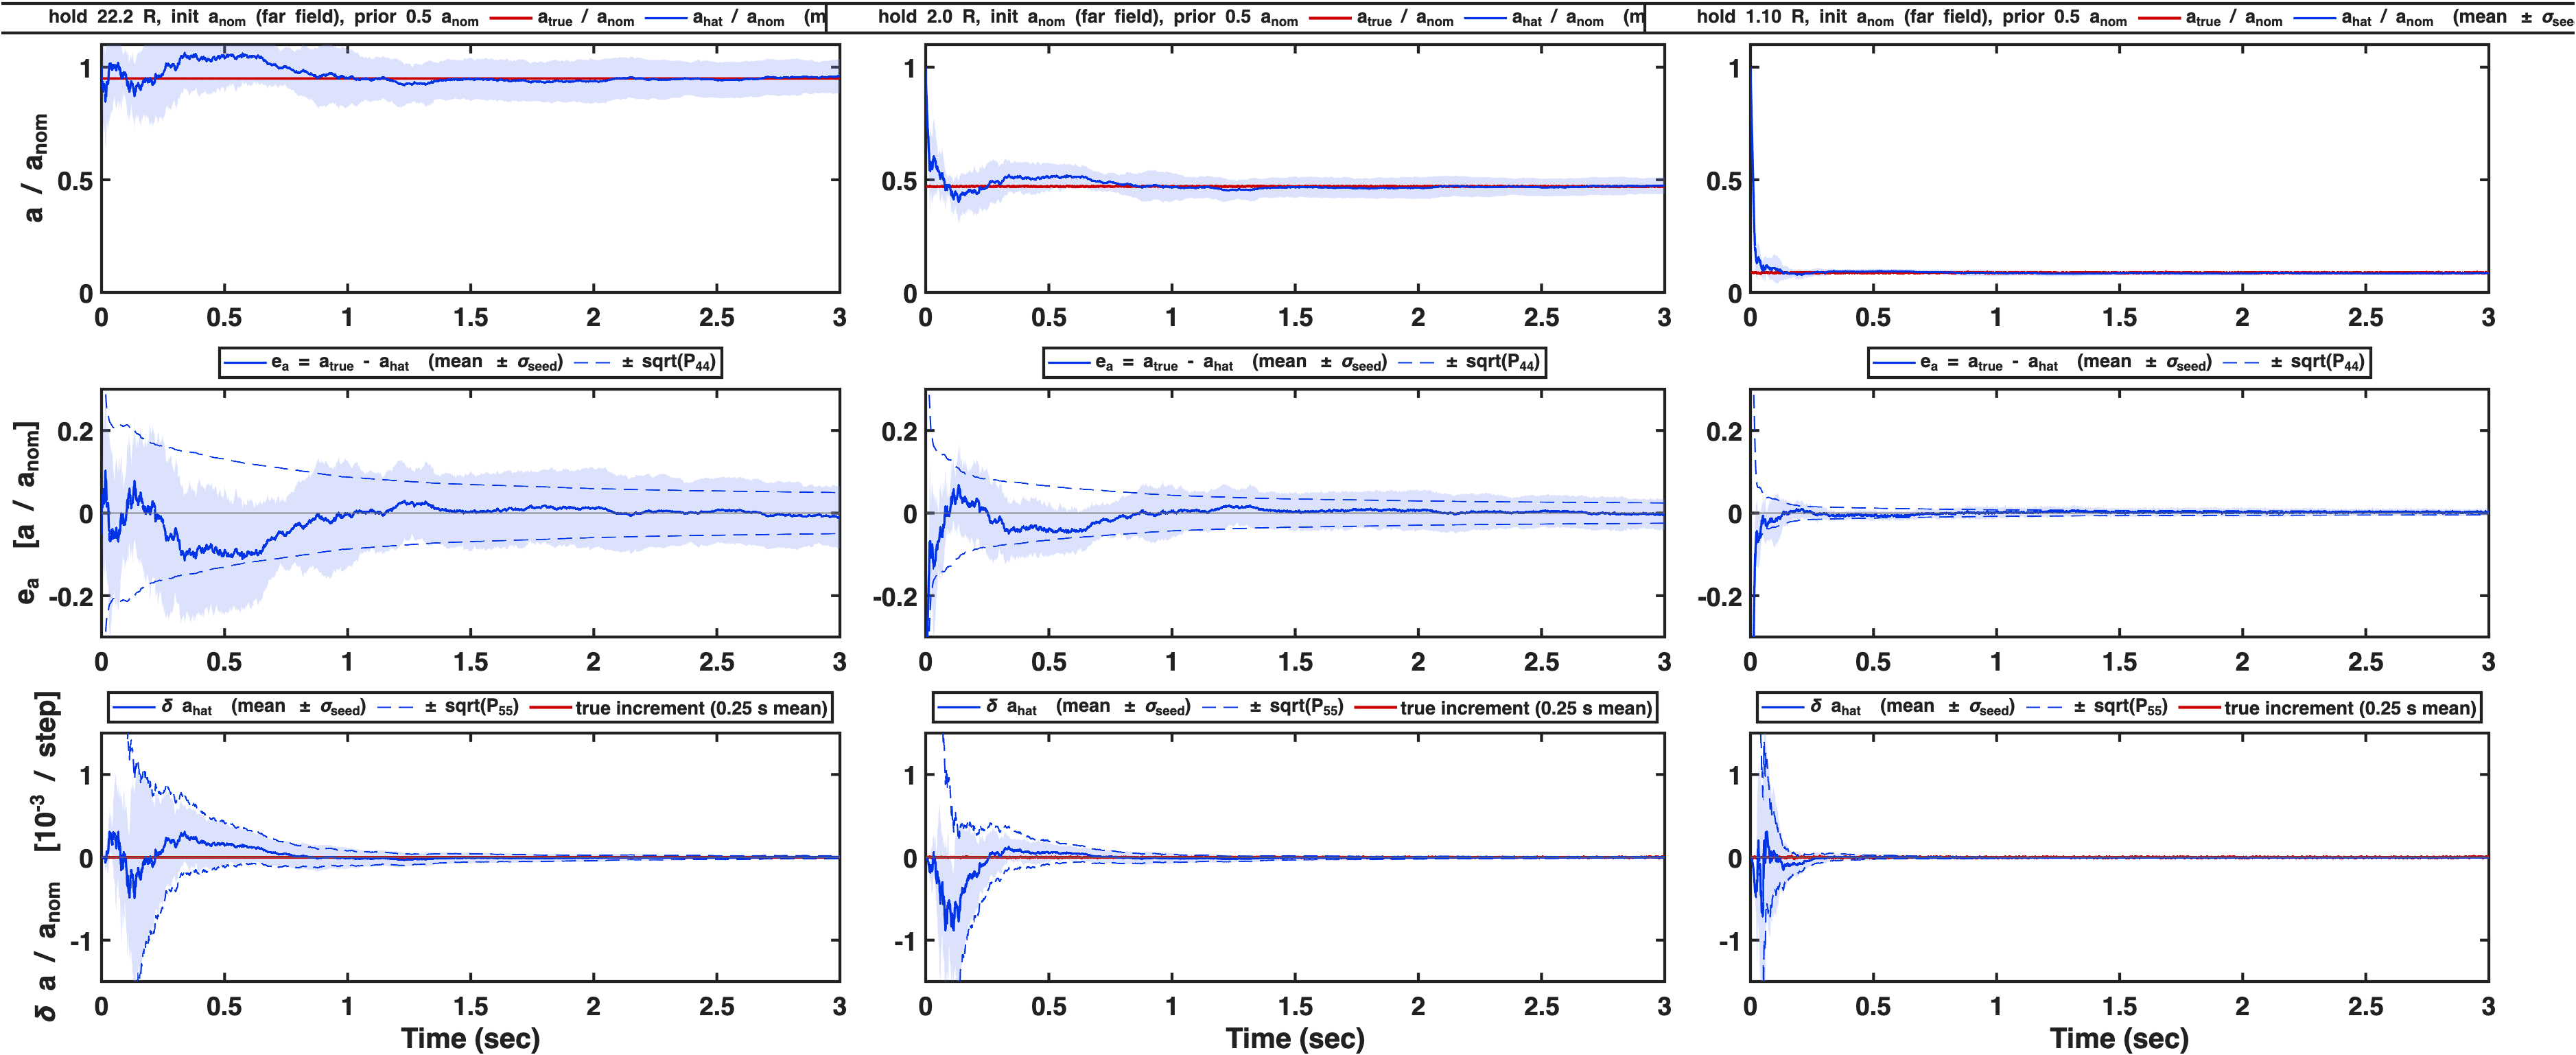
\includegraphics[width=\textwidth]{fig_noap_fixed.png}\end{center}
\textit{Fixed heights, far-field init $\hat a_x[0] = a_{nom}$: rows = gain, error with $\pm\sqrt{P_{44}}$, rate. Level converges at every height (last-second mean error $\le 0.2\%\,a_{nom}$); the rate slot dies within 0.5 s.}

\hd{13. The two honesty gaps, discriminated (\texttt{probe\_5state\_noap\_honesty.m})}
\textbf{Gap 1, hold $P$ 1.5--1.8$\times$ overconfident.} Not the metric: against $a_{det}(\bar h_d)$ the ratio is unchanged (1.53 at 22.2 R where $a_{ram} \equiv 0$). Not the filter: with a white Gaussian oracle $u$ of the same mean and marginal (IF = 1) the ratio is \textbf{0.96}. The measured colour of the real $u$ ($\rho_u = 0.65, 0.36, 0.13, \dots$, $1 + 2\sum\rho = 3.63$) matches the booked $\mathrm{IF}_{white} = 3.75$, so the DC factor is right and the residual is what ``white with inflated $R$'' cannot represent: a correlated sample stream feeding a two-slot (level + rate) filter. Next instrument, not tuning: an explicit MA/AR model of $u$ in the measurement equation (Meng ledger 40 \texttt{y2\_ma2} precedent).

\textbf{Gap 2, $y_1$ 1.76 in the oscillation.} In 0.25 s bins the ratio is 2.0--2.8 exactly where $e_a \approx -0.3$ ($\hat a_x$ below the truth at the gain peaks) and 0.5--0.75 where $e_a > 0$; the bin values follow $a_x/\hat a_x$ (e.g. 0.62/0.29 = 2.1 vs 2.35 measured), i.e. the thermal container $Q_T = 4k_BT\hat a_x$ evaluated at a gain that is wrong by 2--3$\times$. Evaluating $Q_T$ at $a_x$ (\texttt{q\_gain\_true}) moves the window ratio 1.76 $\to$ 1.53 and makes descent / hold-end honest (1.04 / 1.05); the oracle $y_2$ changes nothing; the true-gain law does not remove it (2.09). The remaining 1.5 is [hypothesis] the deterministic $F_{dx} e_a$ swing counted as variance against a $P_{44}$ that is 30$\times$ too small --- the frozen-rate model's own error. Both gaps are consequences of $|e_a| \sim 0.3$, i.e. of \S 10 item 4, not separate defects.

\newpage
\begin{center}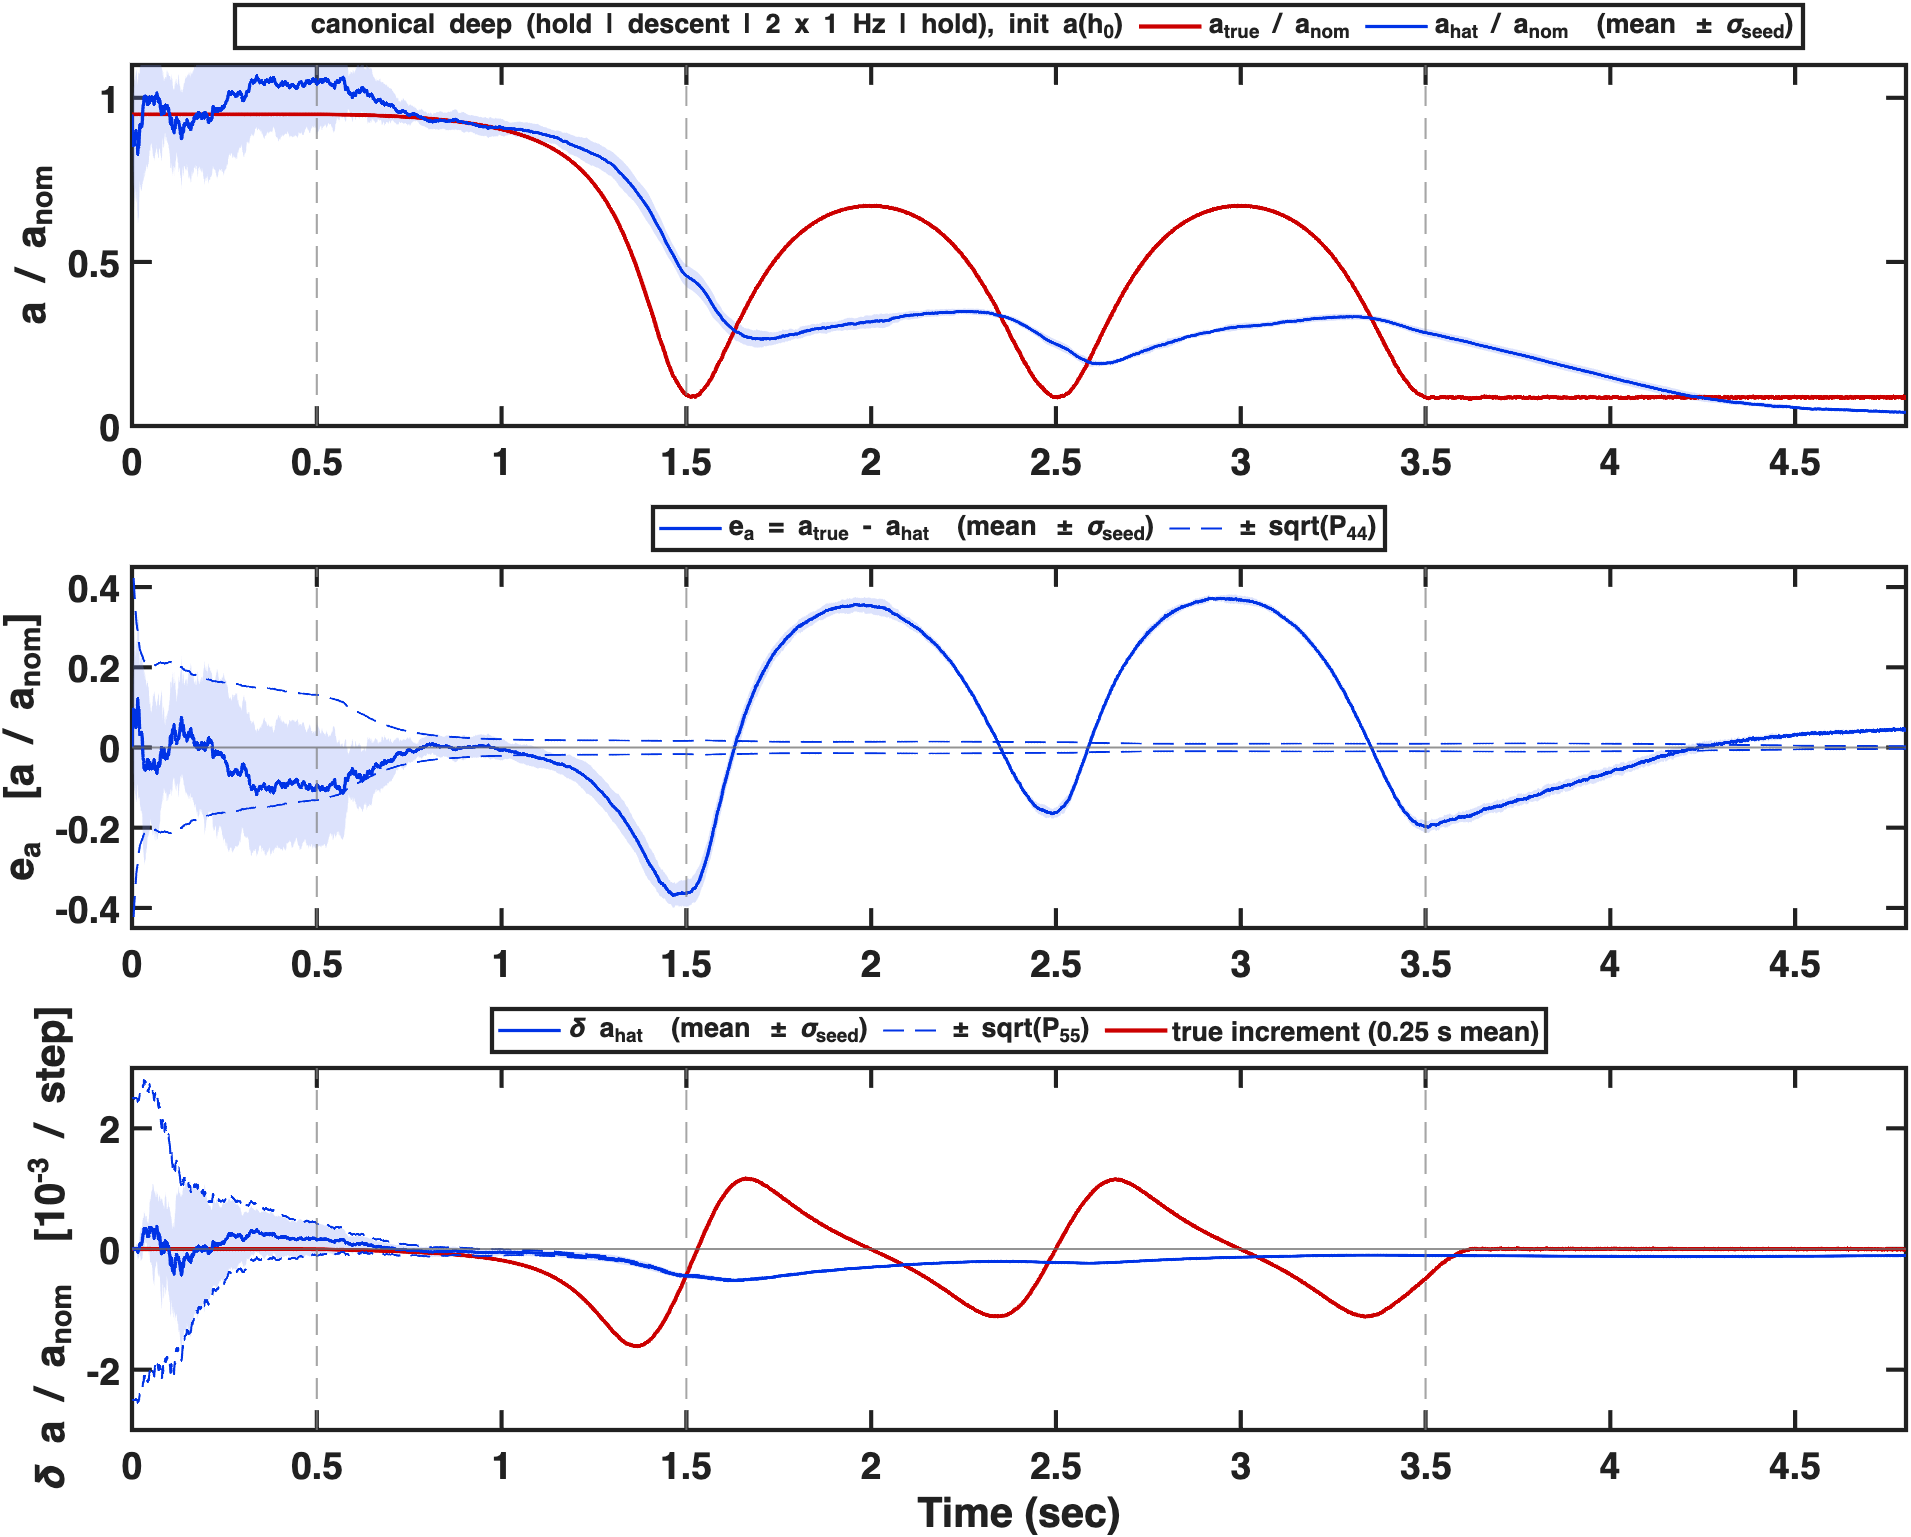
\includegraphics[width=0.9\textwidth]{fig_noap_canon.png}\end{center}
\textit{Canonical deep trajectory, cheat init: the rate estimate (row 4, blue) stays at zero while the true increment swings $\pm 2\times10^{-3}$ per step; the level follows through the $y_2$ row only, as a low-pass of the swing (row 3, $\pm 0.35\,a_{nom}$, $\sqrt{P_{44}} = 0.01$).}

\newpage
\begin{center}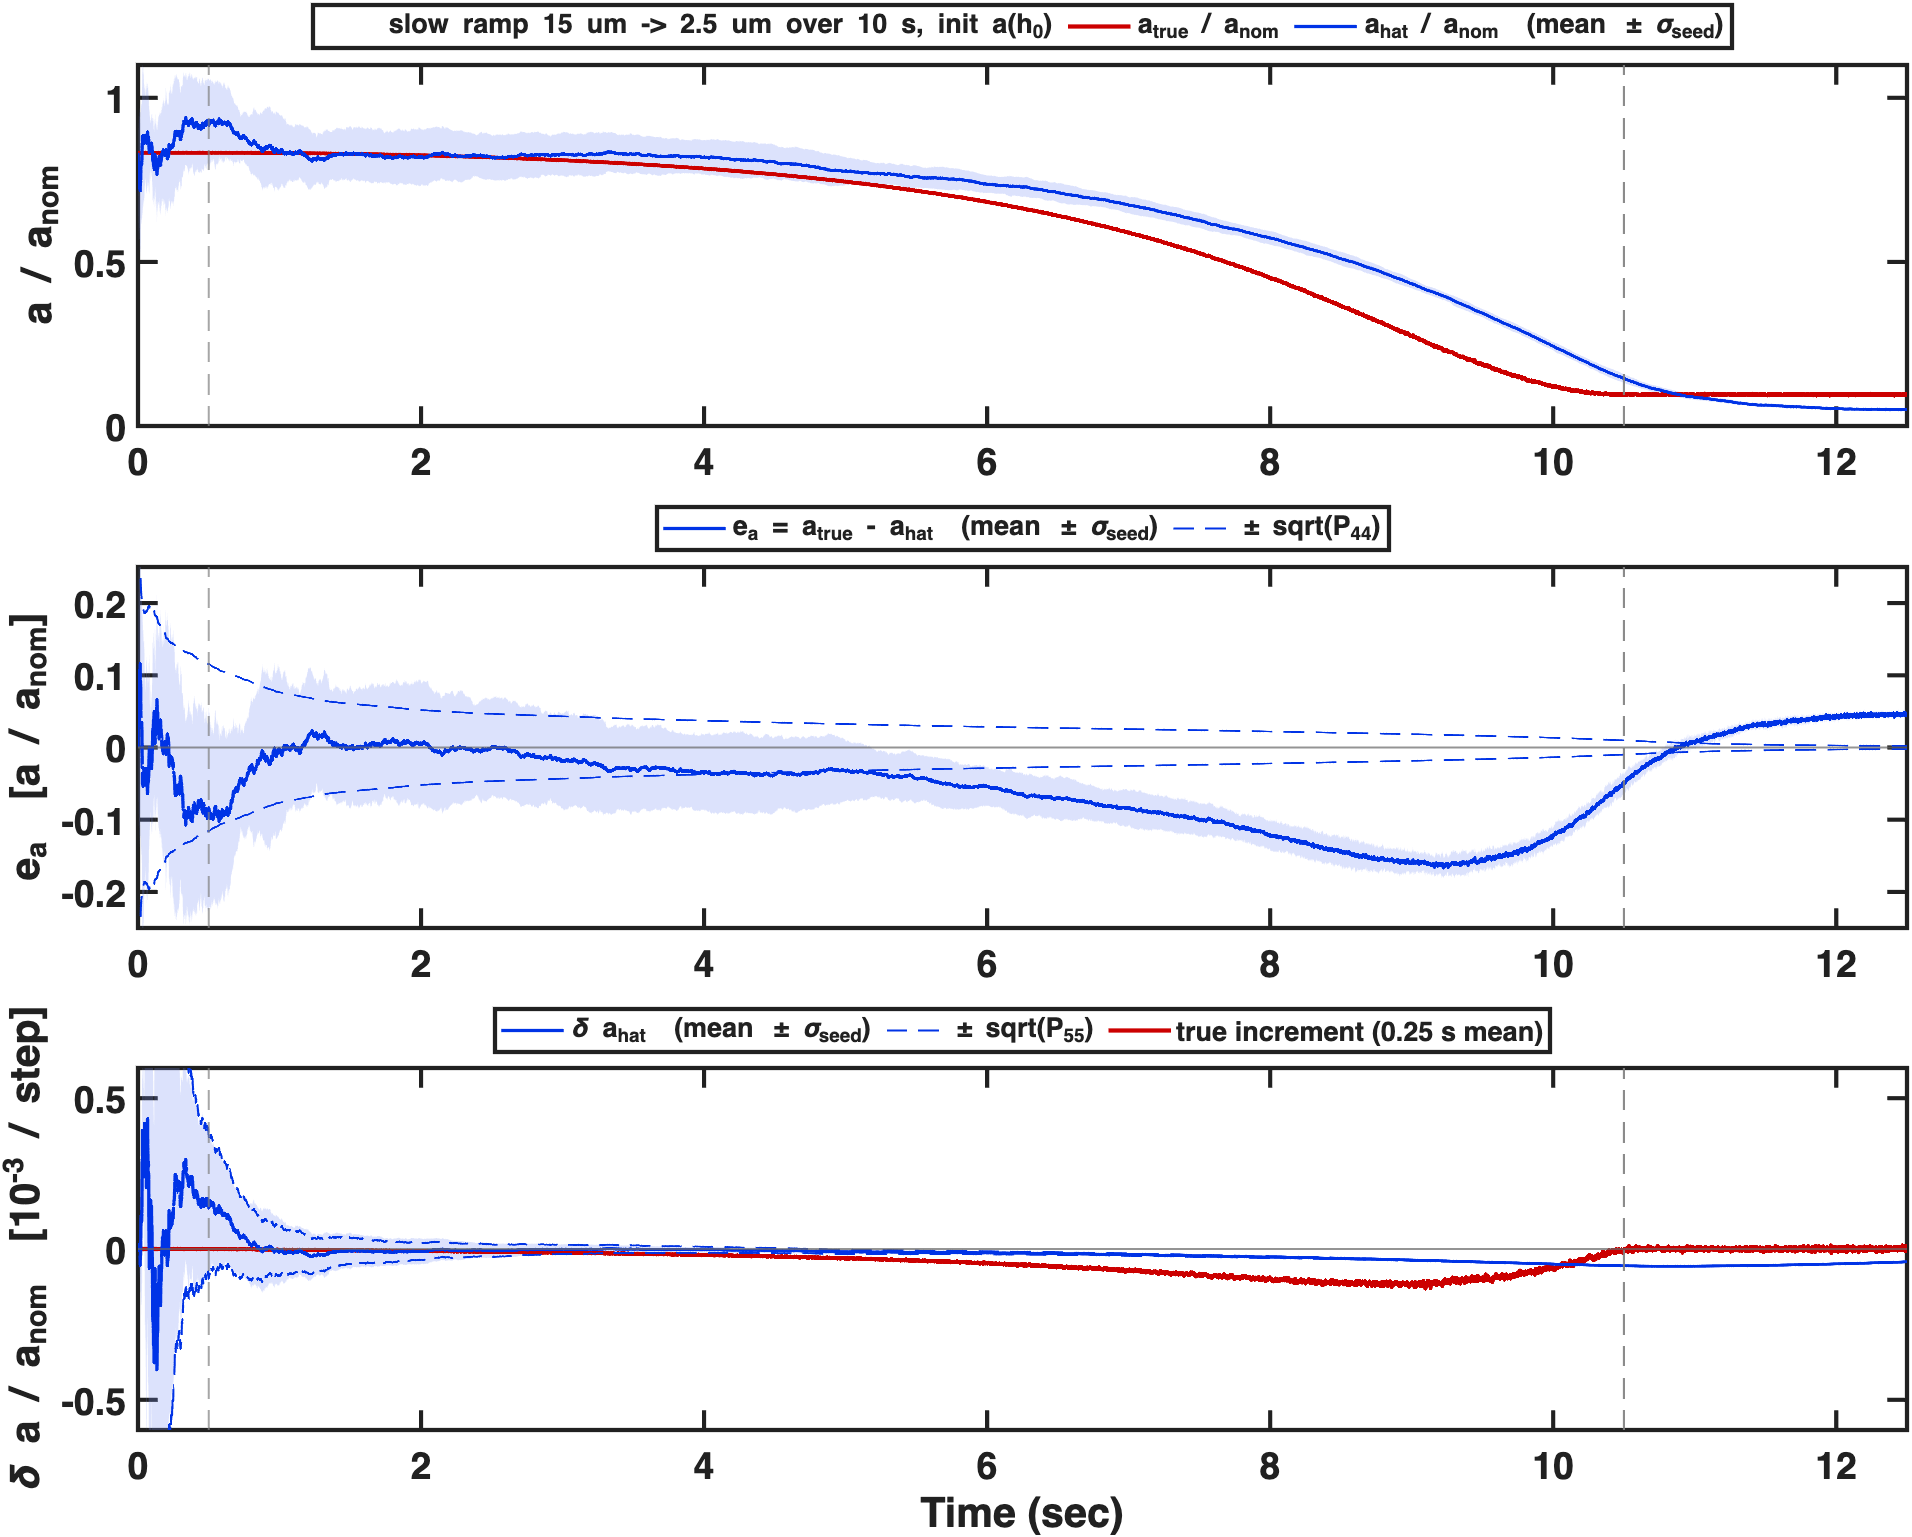
\includegraphics[width=0.9\textwidth]{fig_noap_meng.png}\end{center}
\textit{Slow ramp (15 to 2.5 $\mu$m over 10 s): lag builds to $+0.17\,a_{nom}$ at the ramp end and relaxes to $-0.02$ in the hold; the rate slot never carries the ramp.}

\newpage
\hd{14. Slow ramps and the forgetting factor (2026-09-21; \texttt{run\_5state\_noap\_slow.m}, 5 seeds)}
House ramp 15 $\to$ 2.5 $\mu$m over $T_d \in \{10, 20, 40\}$ s. Pure layer 1: the lag error peak is $-0.17 / -0.17 / -0.16\,a_{nom}$ at all three speeds, because the level channel's time constant grows with the record ($\tau$ = 0.90 / 1.74 / 3.14 s, $P_{44} \propto 1/N$): slowing the command does not help a filter with infinite memory, $\tau\cdot\dot a$ stays put. $\sqrt{P_{55}}$ at the fastest fall is 50--150$\times$ below the true increment.

\textbf{Layer 1.5 = gain-block forgetting} $\lambda_f$ (slots 4--5 of $P$ divided by $\lambda_f$ before each predict; a memory knob, $T^* = T_s/(1-\lambda_f)$): 0.9995 ($T^* = 1.25$ s) gives lag peak $-0.065 / -0.056 / -0.035$, $\tau \approx 0.2$ s, rate slot alive (row 3), hold-end honesty 1.09 / 0.93 / 0.70; 0.998 ($T^* = 0.31$ s) buys no further lag reduction and doubles the hold-end scatter (0.009 vs 0.005). Tracking rms on the ramp 25 nm in every cell: the gain error never reaches the position (06-18). The first-second transient ($\pm 0.1$, \S 13) is unchanged by $\lambda_f$.
\begin{center}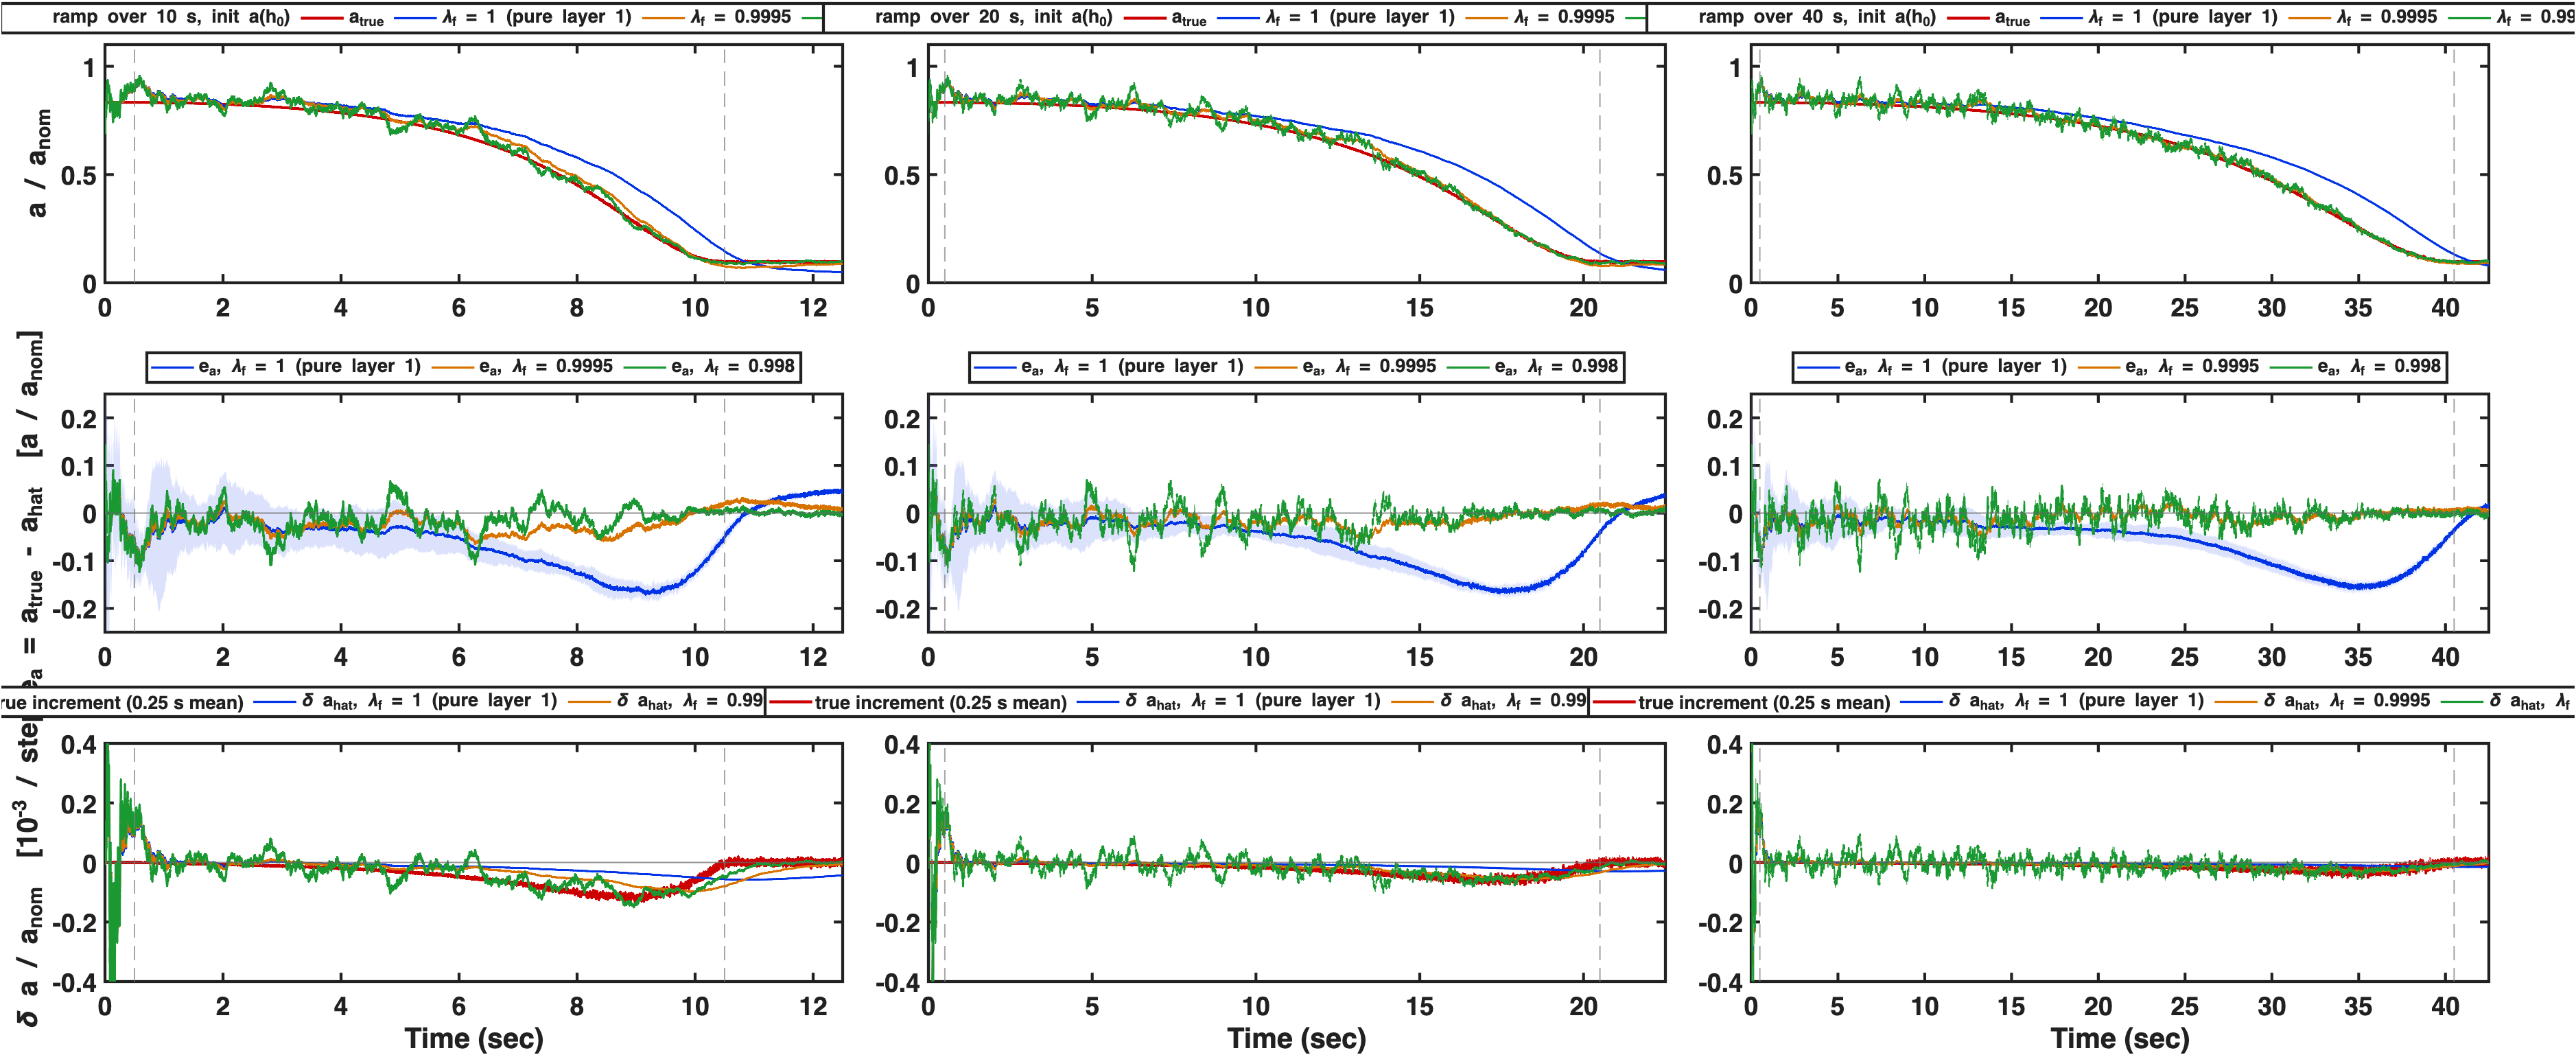
\includegraphics[width=\textwidth]{fig_noap_slow.png}\end{center}
\textit{Columns $T_d$ = 10 / 20 / 40 s; rows gain, $e_a = a_{true} - \hat a$, rate. Blue = pure layer 1, orange $\lambda_f = 0.9995$, green $0.998$.}

\newpage
\hd{15. Closing state of the layer (2026-09-22)}
\textbf{Final defaults} (all in the controller): gain model order 2 (level + rate), $Q_{44} = Q_{55} = 0$; memory schedule \texttt{lf\_mode = 'ljung'} on the gain block (slots 4, 5, 8), clamp $\lambda_f \ge 0.98$ ($T^* \ge 31$ ms; the 1 Hz canon asks for $\sim$30 ms, the slow ramp pays 5.0 $\to$ 5.3\% rel. rms); $\sqrt{P_{44}[0]} = 0.5\,a_{nom}$ (far-field seed) / $0.05\,a_{nom}$ (cheat seed); $\sqrt{P_{55}[0]} = a_{nom}/40000$ (runs start in a hold; $a_{nom}/400$ let the first correlated samples be read as a slope: start transient $\pm 0.09 \to \pm 0.02$, ramp and hold unchanged).

\textbf{Five-cell battery, plane, 10 seeds} (\texttt{run\_5state\_noap\_battery} tag \texttt{\_best}; figures below): fixed 22.2 / 2.0 / 1.10 R last-second mean $\le 0.002$, seed sd 0.051 / 0.033 / 0.008 vs $\sqrt{P_{44}}$ 0.043 / 0.025 / 0.005 (honesty 1.2 / 1.3 / 1.5); slow ramp descent $-0.015 \pm 0.037$ ($\sqrt{P_{44}}$ 0.044), hold-end $-0.002 \pm 0.008$ (1.02); canon oscillation $+0.05 \pm 0.05$ ($\sqrt{P_{44}}$ 0.07), hold-end $-0.002 \pm 0.010$. Cell wall (plane slid 1.05 R): same absolute levels, relative 5$\times$ smaller (the estimator reads no wall).

\textbf{Variants measured and retired} (5 seeds unless noted): gain order 1 worst on both trajectories (rate slot needed); order 3 canon rms $0.066 \to 0.041$ at hold sd $0.009 \to 0.013$, no gain on the ramp (flag \texttt{gain\_order}); damped rate (Singer, $\rho = 1 - 1/T^*$, $Q_{55} = (1-\rho^2)(r\hat a)^2$) canon rms $\to 0.037$, max $0.143 \to 0.086$, ramp $+14\%$ (flag \texttt{rate\_damp}); forgetting on the rate slot only equal on the ramp, canon rms $0.105$ and hold-end bias $+0.04$ (flag \texttt{lf\_slots}); constant $\lambda_f$ with rate-only forgetting: 0.9995 lags and holds $+0.03$, 0.998 far-field $\pm 0.15$; exact wall slope in $r$ identical to the far-field slope (clamp binds); $Q_{55}$ budget $(ra)^2/T^*$ equal to forgetting; gauge-sensitivity $H_2 \times s_i$ (\texttt{y2\_mirror}) biases the 1.10 R hold by $-0.01$ and breaks the ramp ($0.029 \to 0.130$): kept off.

\textbf{What the layer shows}: at a fixed point the scatter plateaus at 5--9\% of $a$ after 0.5 s and does not fall further; on the slow ramp the scatter sits on the same plateau (the ramp is the fixed point at its 0.4--0.6 s averaging time) and the mean lag is removed by the schedule; on the 1 Hz canon the turning-point spike $\sim 0.09$--$0.15$ is the memory limit on a reversing rate. Slowing the command buys $\text{speed}^{1/3}$. The plateau is not the loop echo (true-gain law: 1.52 $\to$ 1.41 at 1.10 R) and not the filter (white oracle $y_2$: 0.96); it is the readout stream's structure, left as the open item of the layer (a readout noise model, not built). Everything beyond this needs $a'\,\Delta\bar w_d$: the next rung.

\begin{center}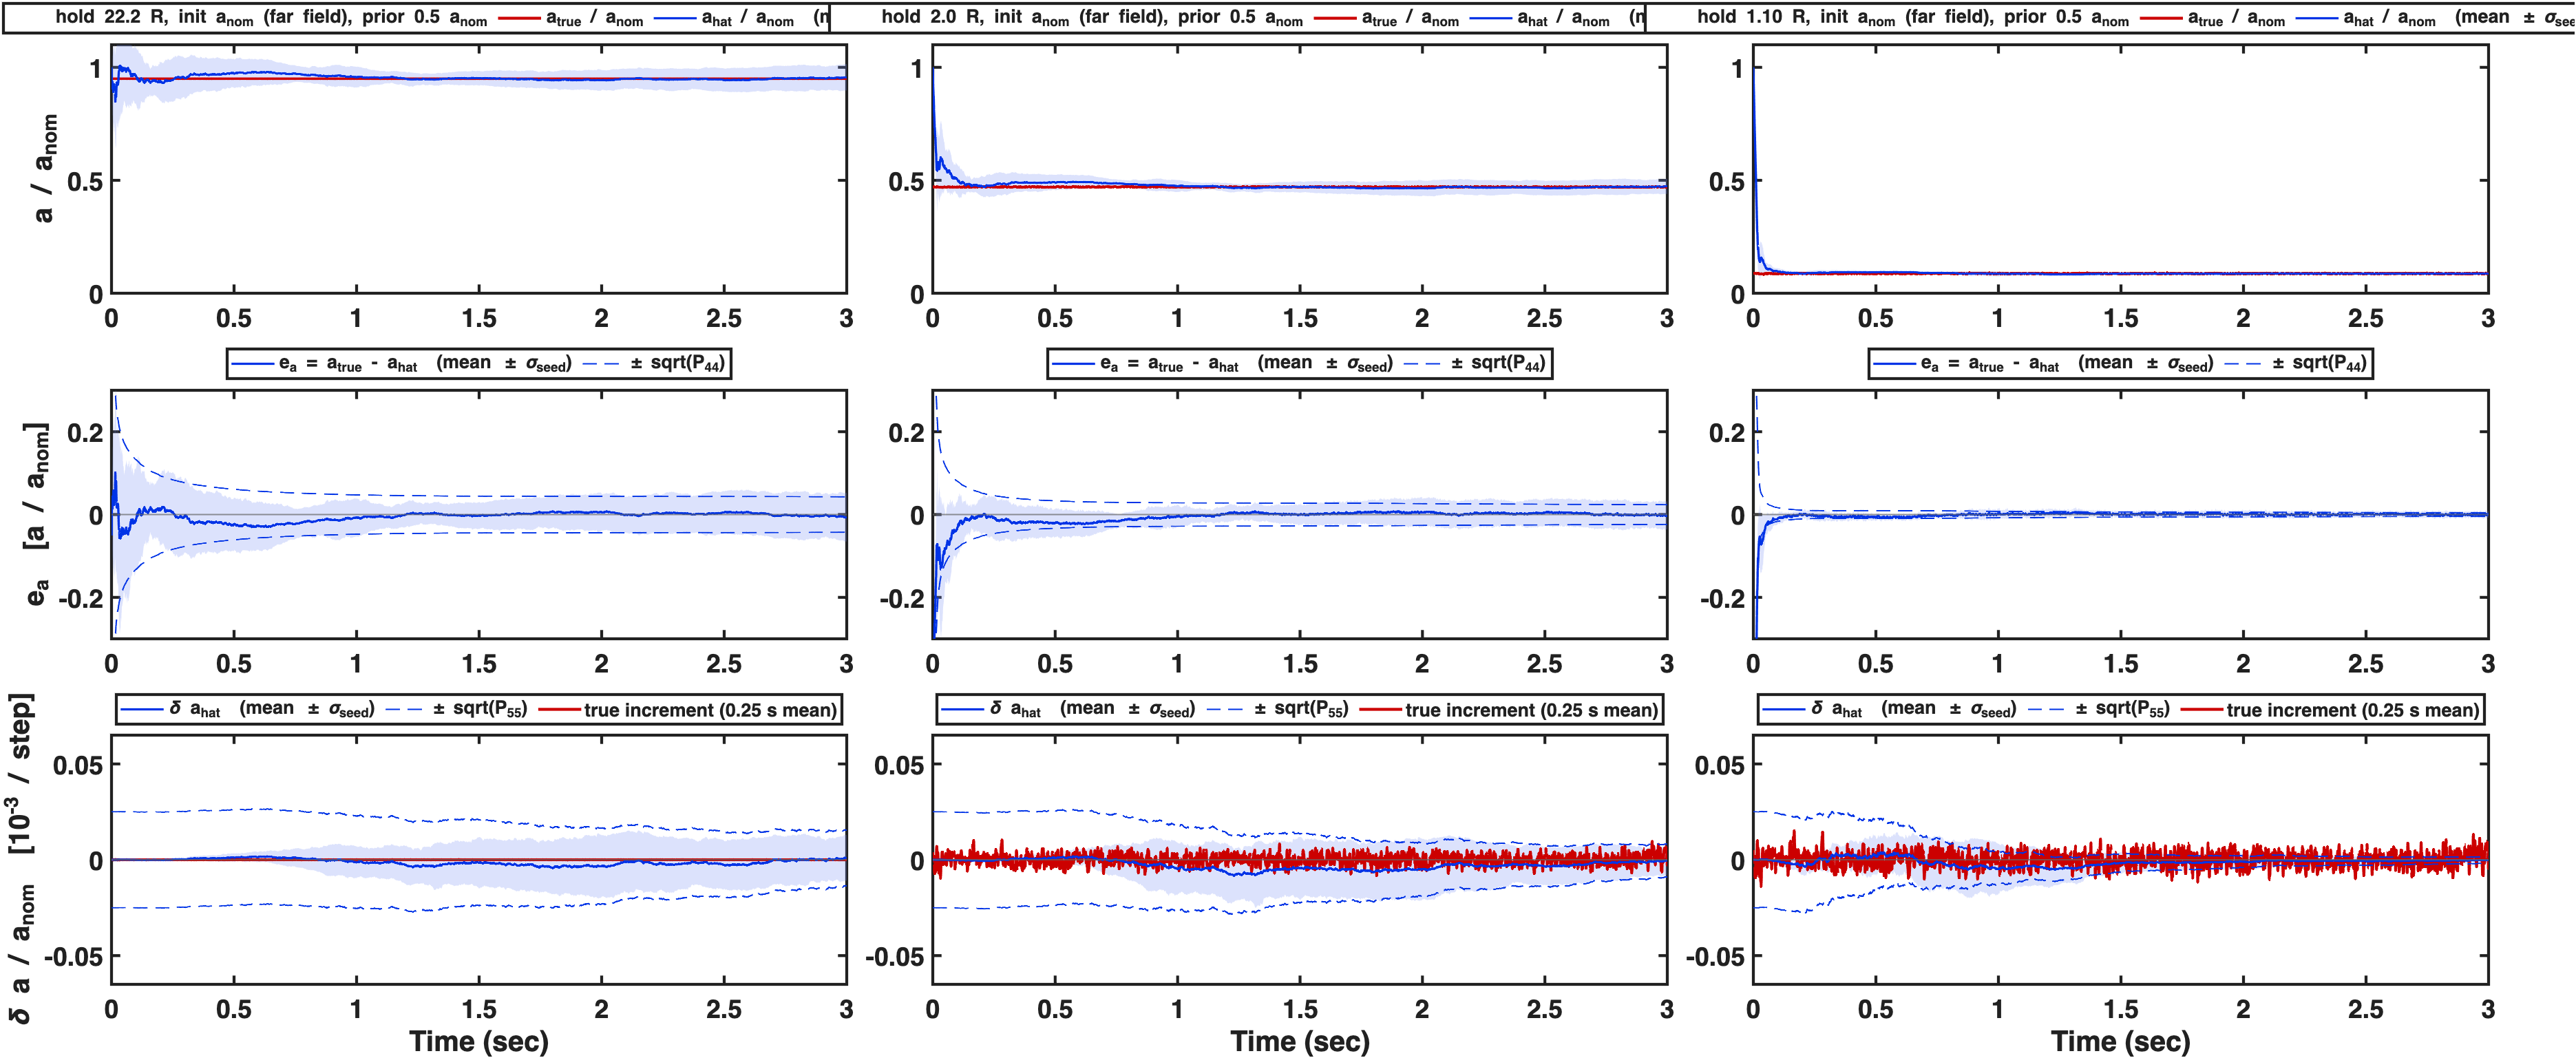
\includegraphics[width=\textwidth]{fig_noap_fixed_best.png}\end{center}
\textit{Final defaults, plane, fixed heights.}
\newpage
\begin{center}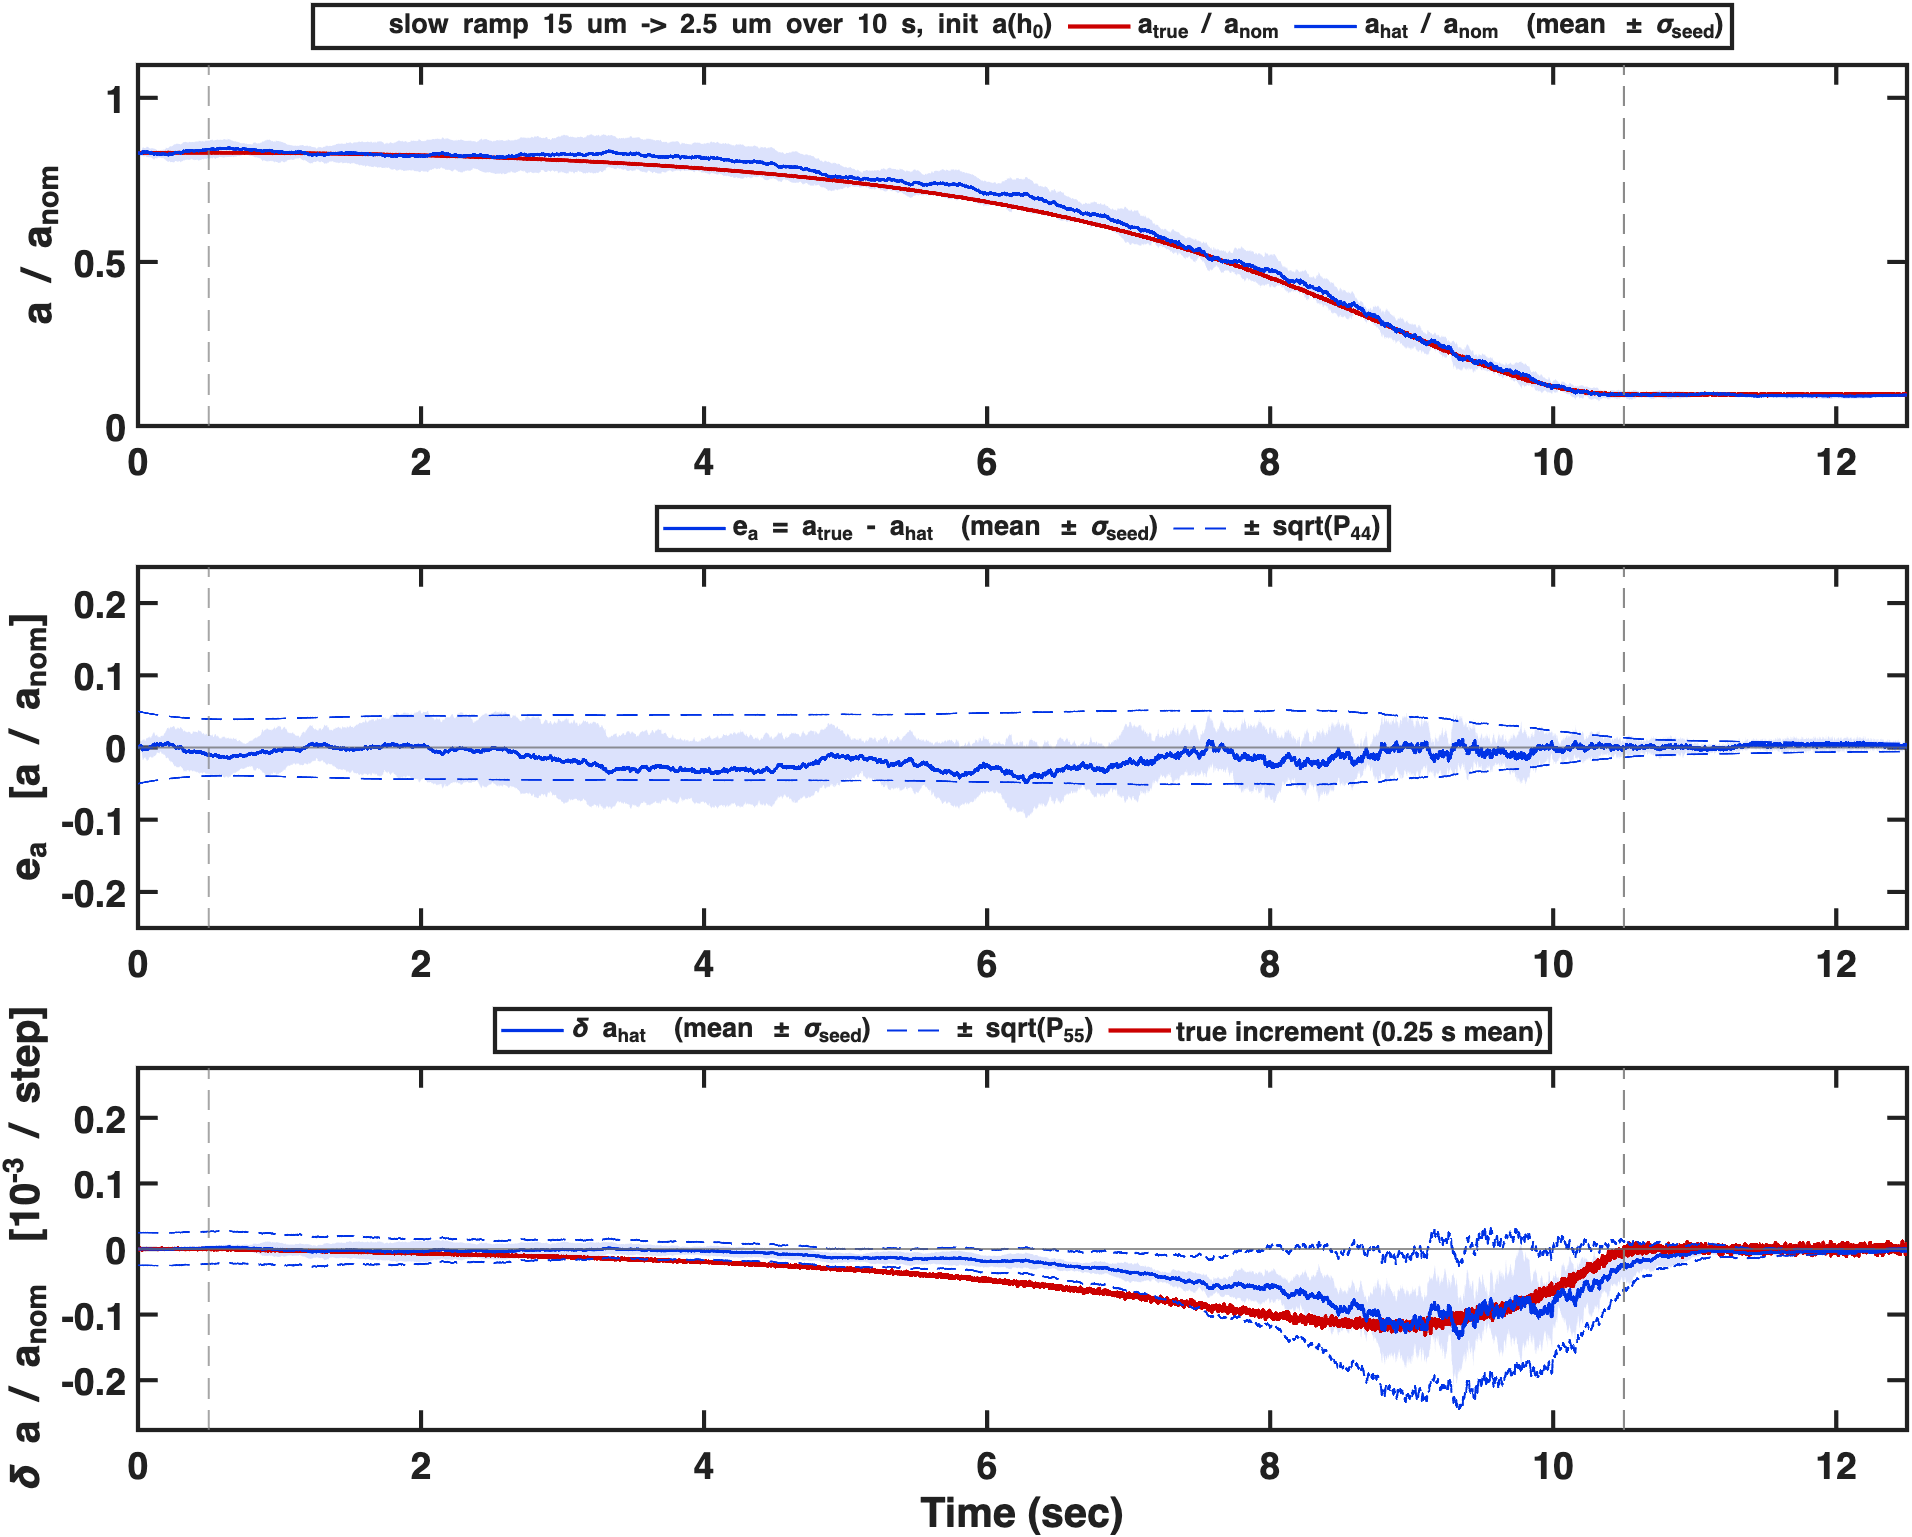
\includegraphics[width=0.85\textwidth]{fig_noap_meng_best.png}\end{center}
\textit{Final defaults, plane, slow ramp.}
\newpage
\begin{center}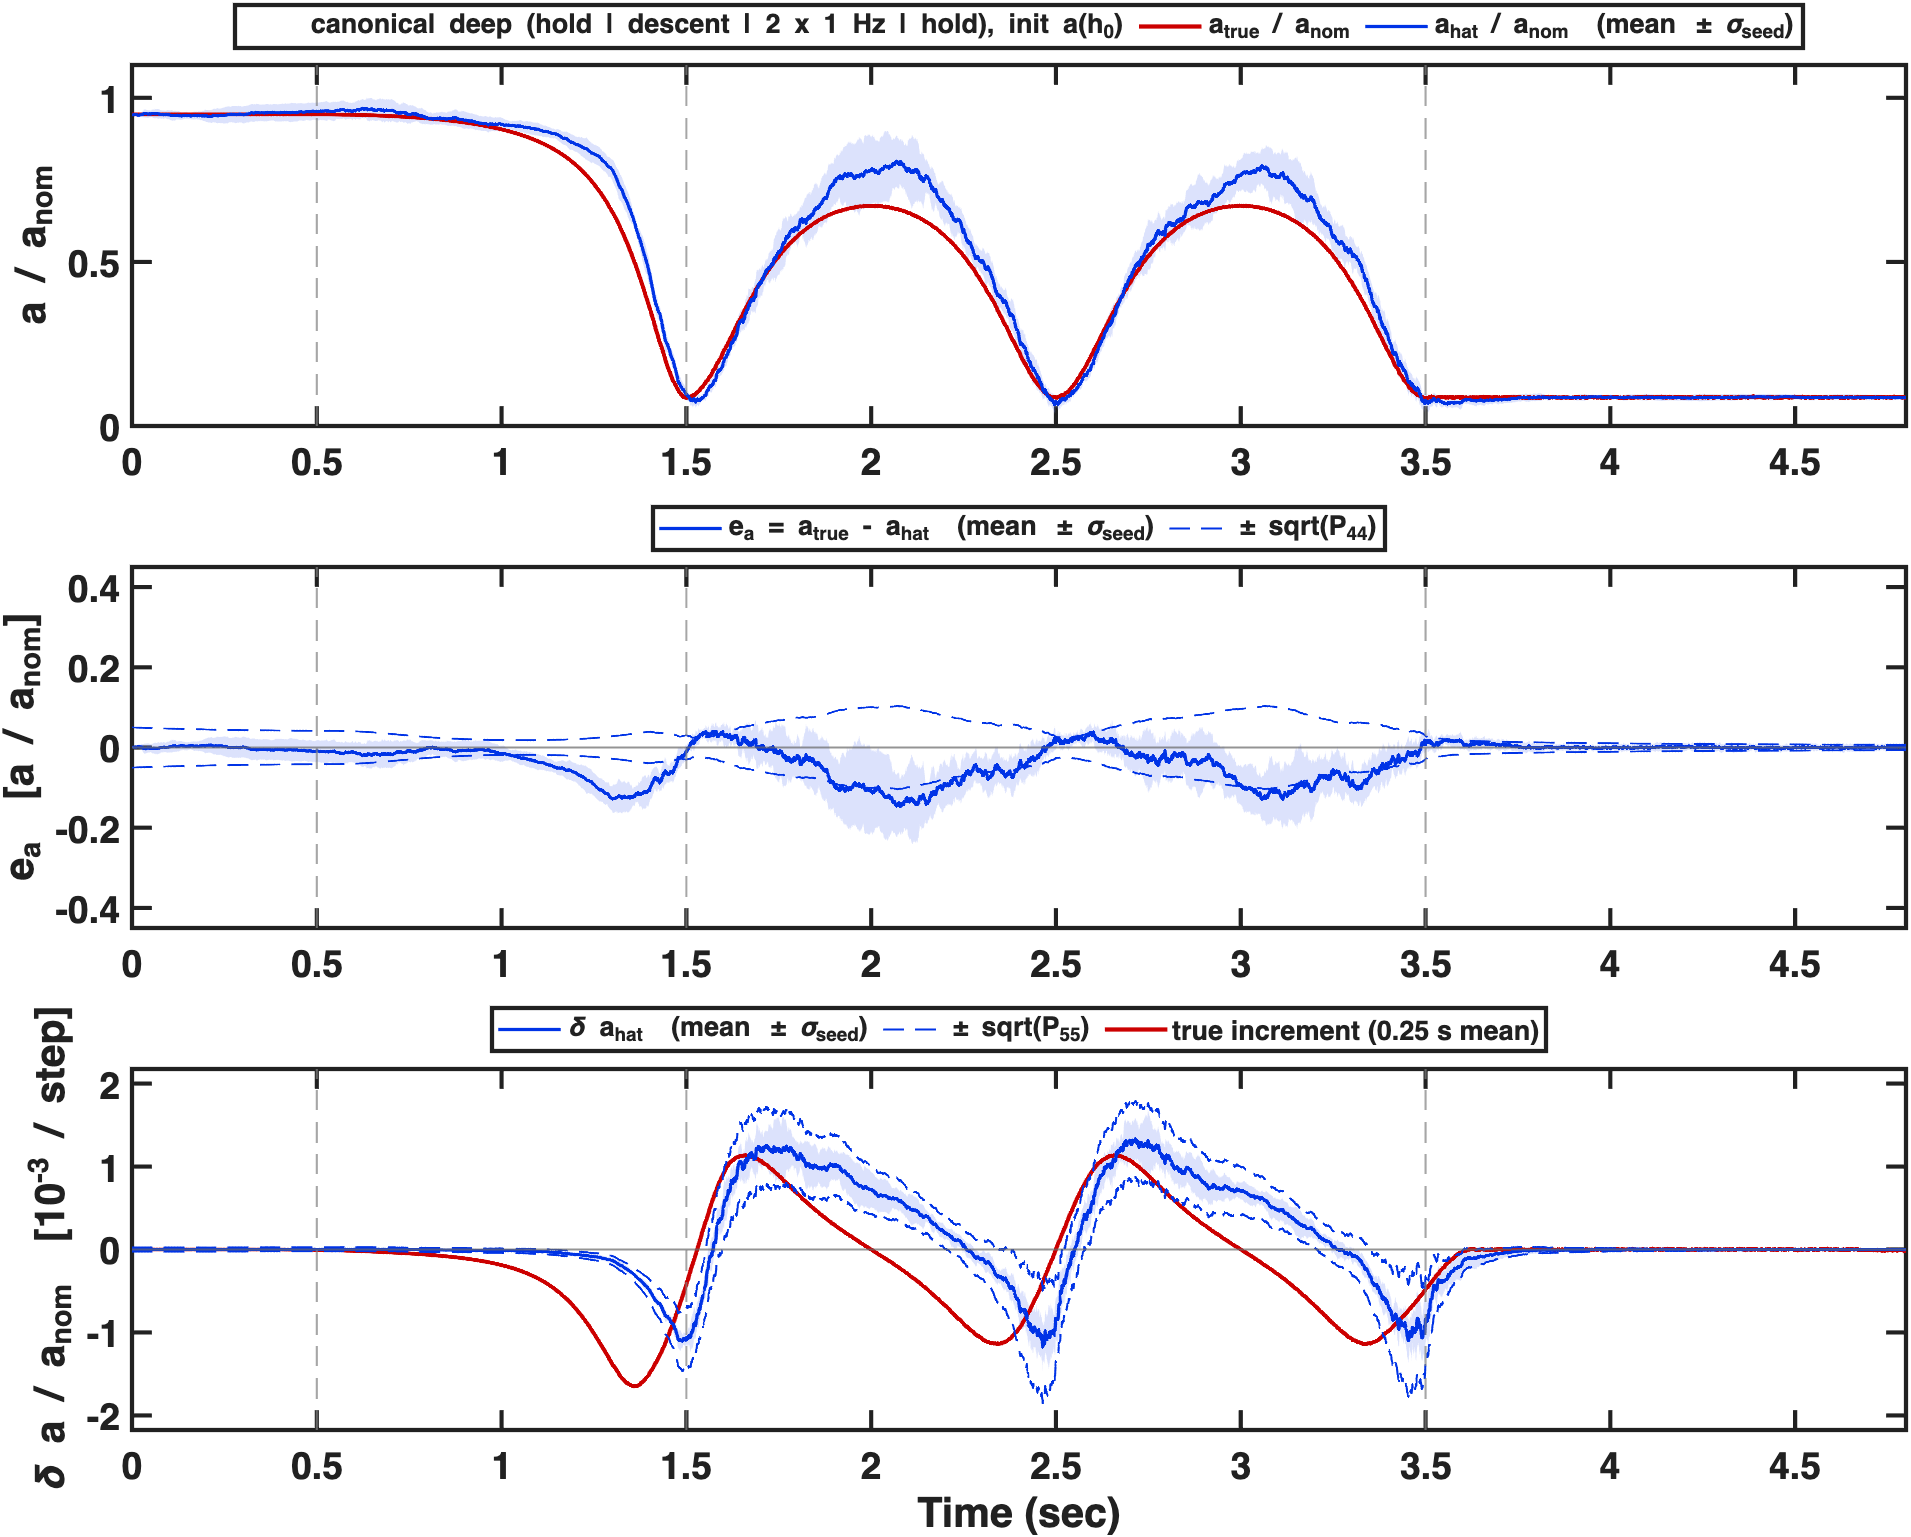
\includegraphics[width=0.85\textwidth]{fig_noap_canon_best.png}\end{center}
\textit{Final defaults, plane, canonical deep.}
\newpage
\begin{center}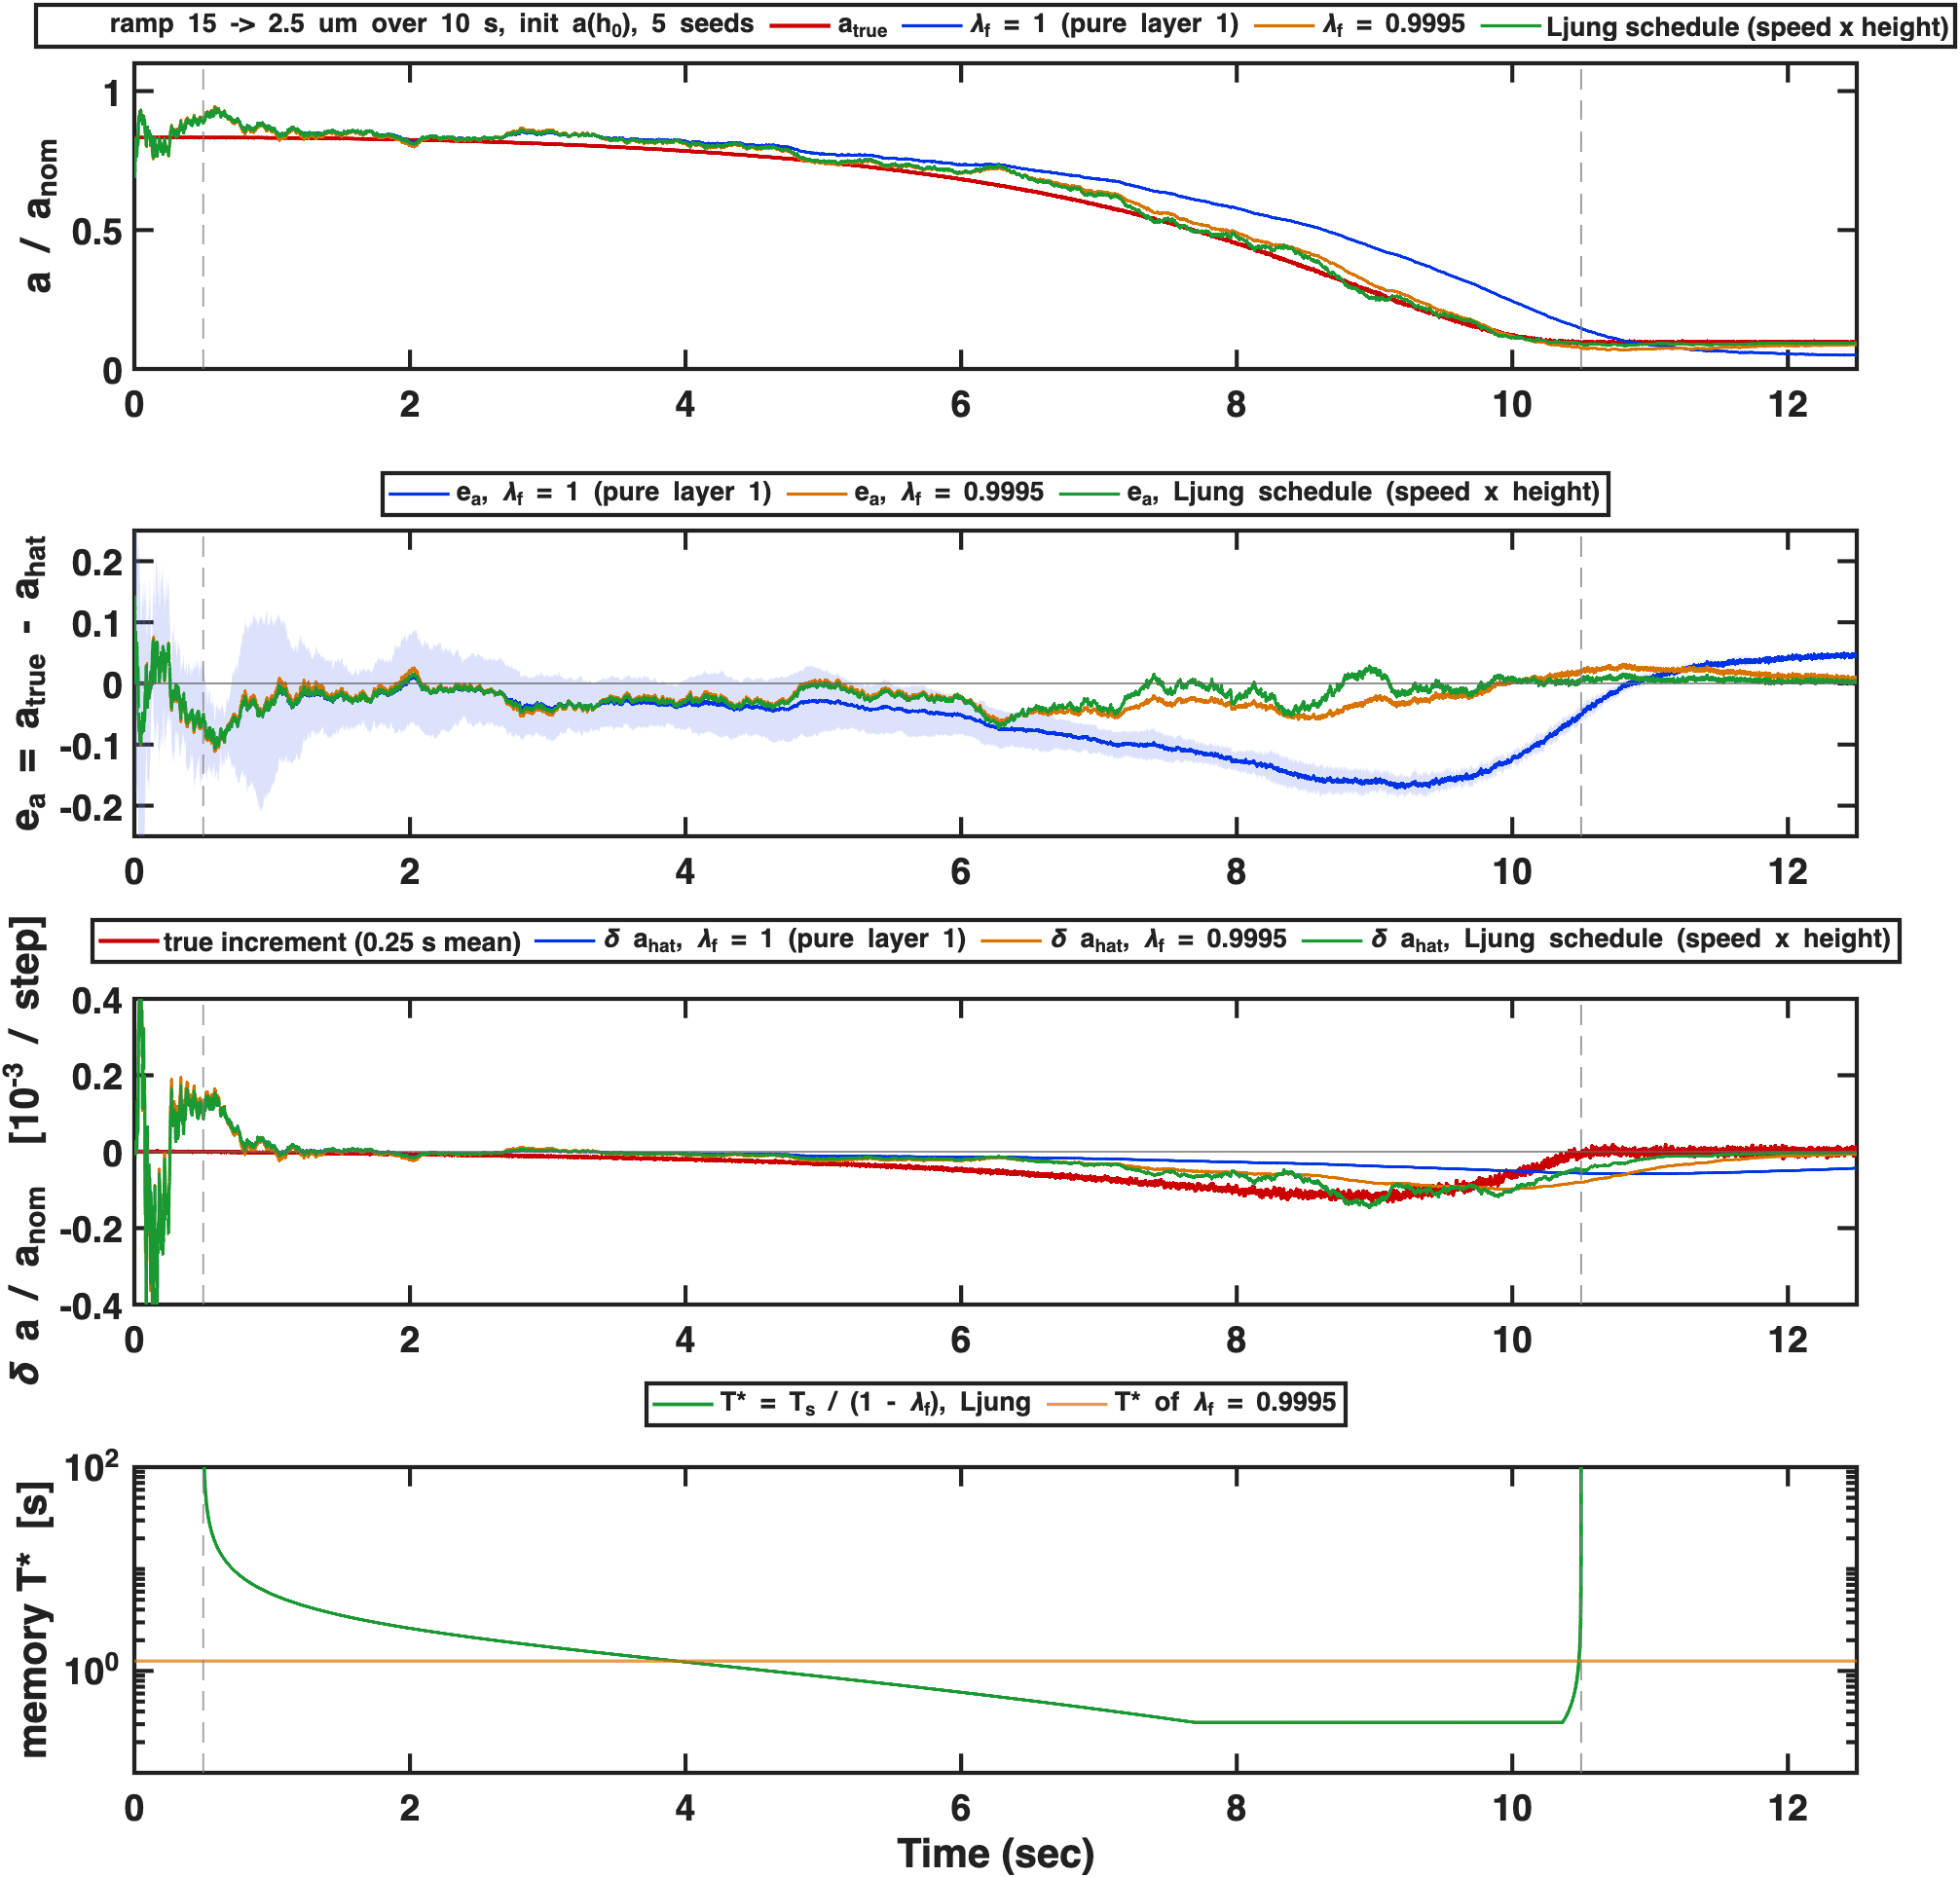
\includegraphics[width=0.9\textwidth]{fig_noap_lfadapt_Td10.png}\end{center}
\textit{Slow ramp: pure layer 1 / constant $\lambda_f$ / Ljung schedule (\texttt{run\_5state\_noap\_lfadapt}).}
\newpage
\begin{center}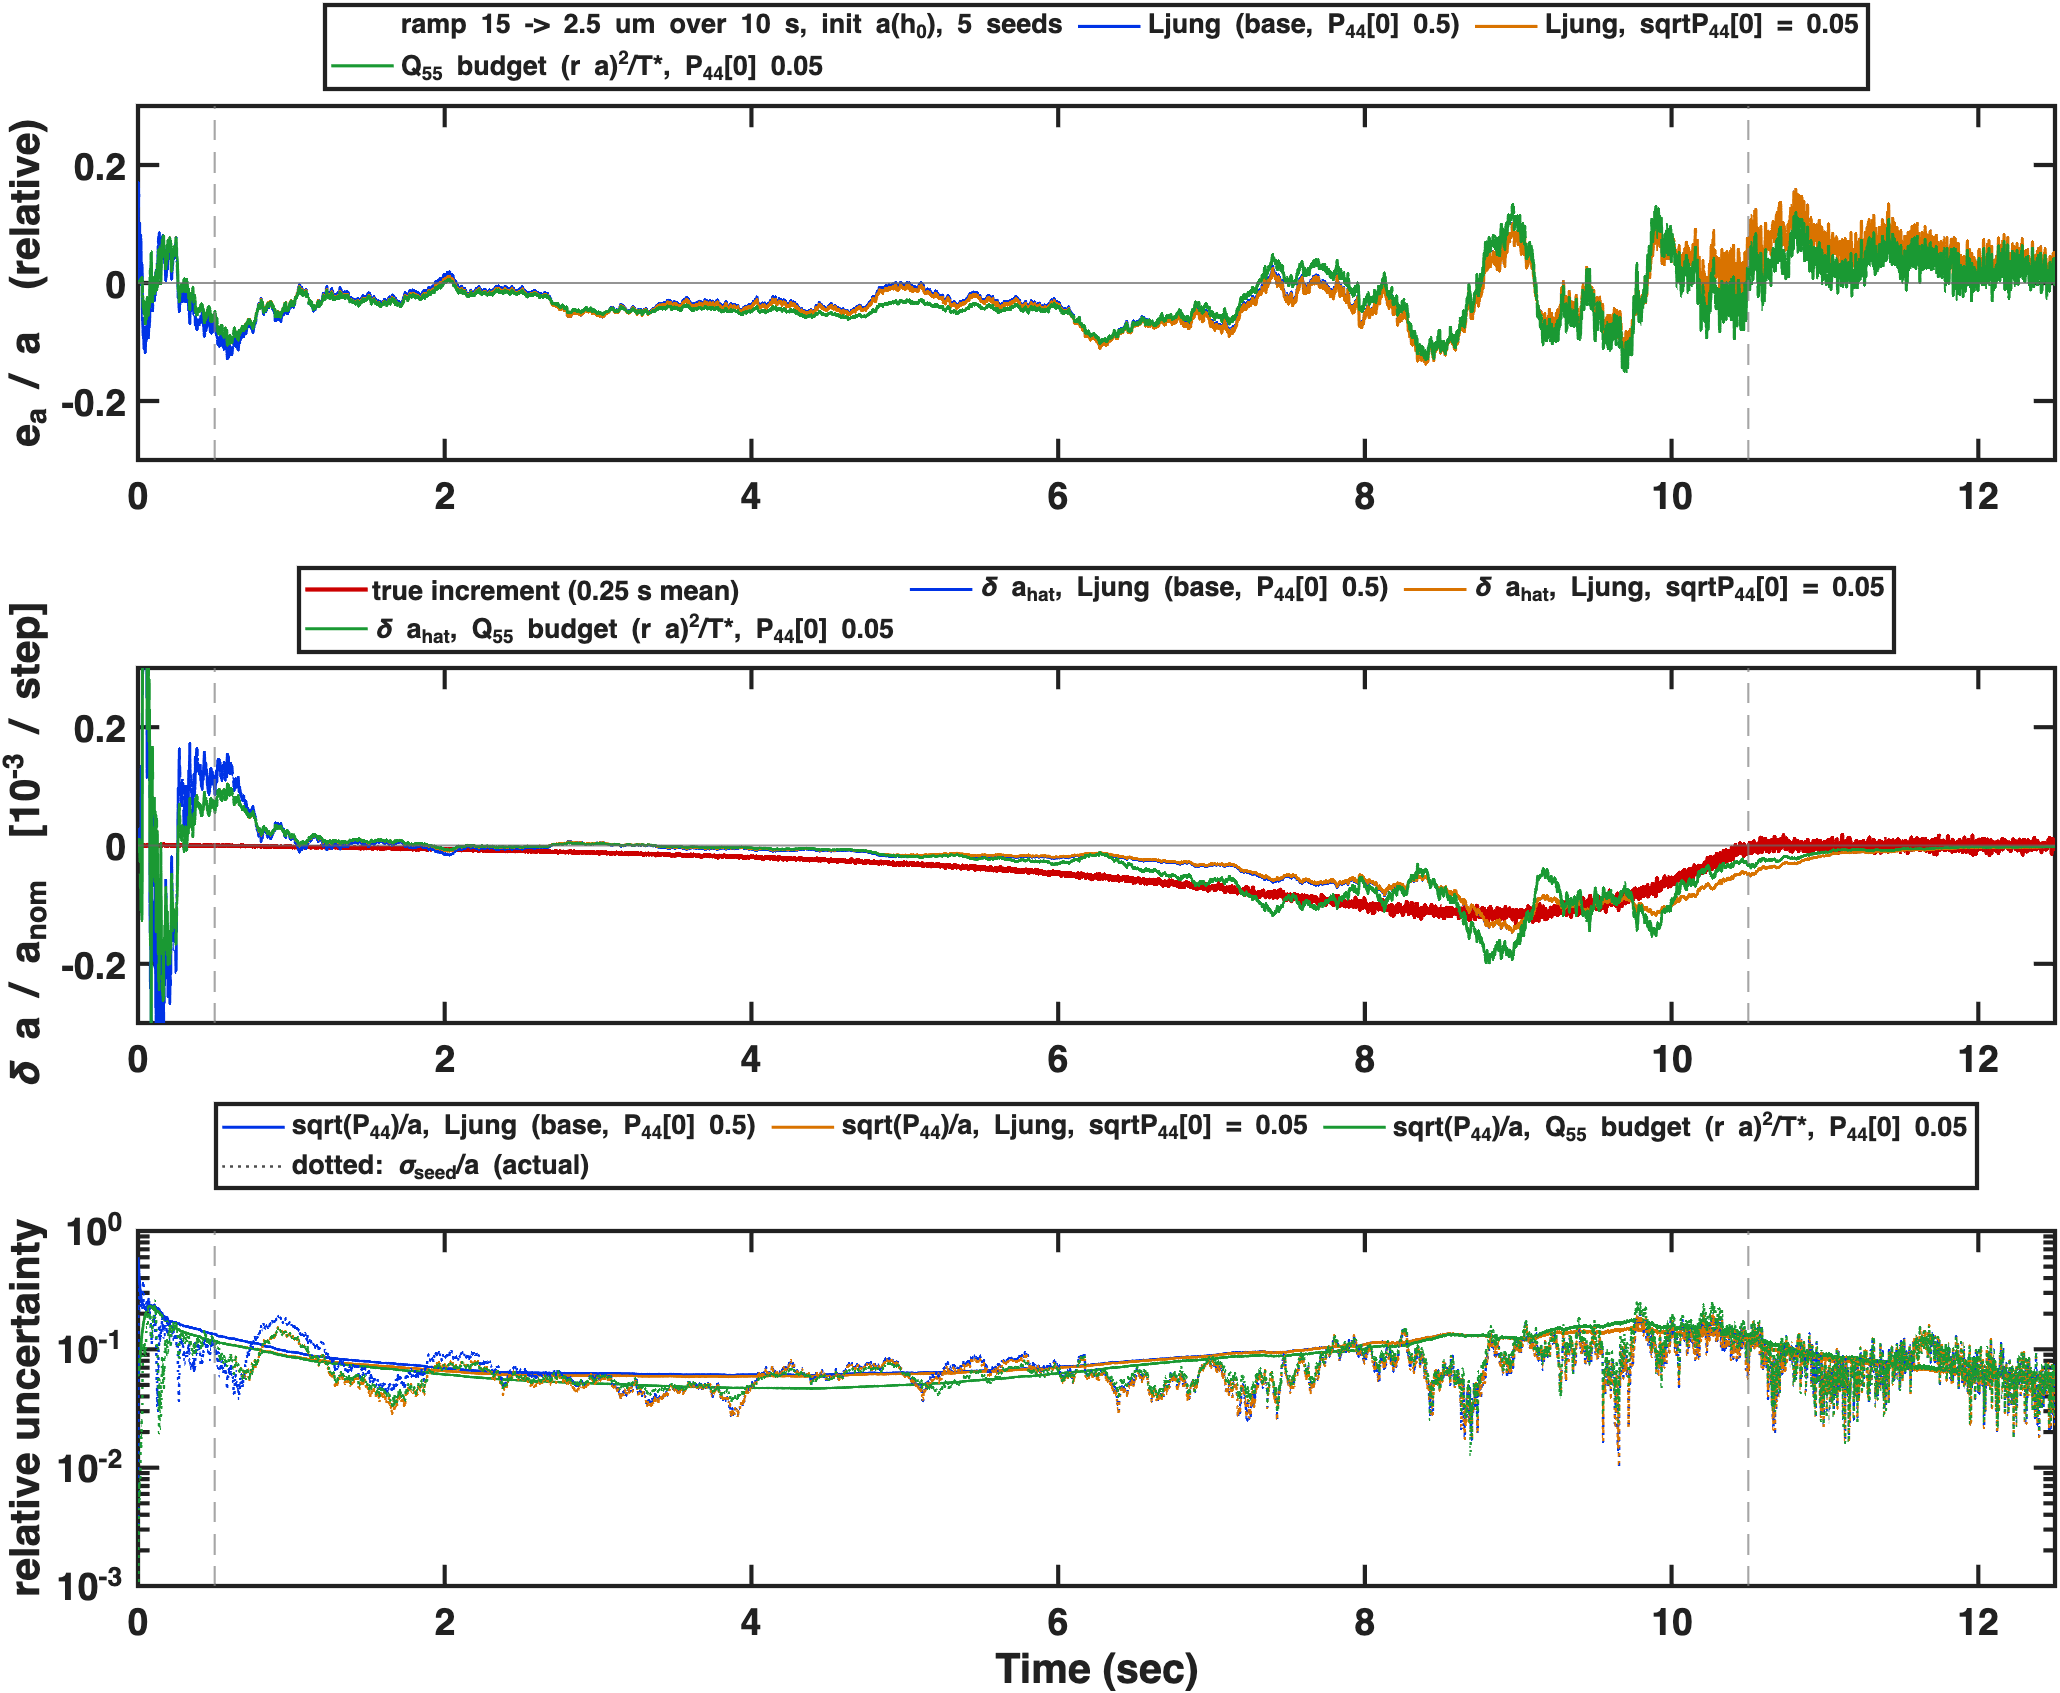
\includegraphics[width=0.9\textwidth]{fig_noap_tune_Td10.png}\end{center}
\textit{Tuning round on the slow ramp (\texttt{run\_5state\_noap\_tune}): $P_{44}[0]$, clamp, exact slope, $Q_{55}$ budget.}

\end{document}
